\section{Pregunta \texttt{b)}}\label{pregunta-b}

\begin{figure}[h]
  \centering
  % This file was created by matlab2tikz.
%
%The latest updates can be retrieved from
%  http://www.mathworks.com/matlabcentral/fileexchange/22022-matlab2tikz-matlab2tikz
%where you can also make suggestions and rate matlab2tikz.
%
\begin{tikzpicture}

\begin{axis}[%
width=0.856\textwidth,
height=0.2\textheight,
at={(0\textwidth,0\textheight)},
scale only axis,
xmin=0,
xmax=10,
xlabel style={font=\color{white!15!black}},
xlabel={Tiempo $[\unit{s}]$},
ymin=-1,
ymax=28,
ylabel style={font=\color{white!15!black}},
ylabel={$\verd{v_{i}}(t)\ [\unit{V}]$},
axis background/.style={fill=white},
title style={font=\bfseries},
title={Entrada al sistema $\verd{v_{i}}(t)$}
]
\addplot [color=Green, forget plot]
  table[row sep=crcr]{%
0	0\\
0.01	0\\
0.02	0\\
0.03	0\\
0.04	0\\
0.05	0\\
0.06	0\\
0.07	0\\
0.08	0\\
0.09	0\\
0.1	0\\
0.11	0\\
0.12	0\\
0.13	0\\
0.14	0\\
0.15	0\\
0.16	0\\
0.17	0\\
0.18	0\\
0.19	0\\
0.2	0\\
0.21	0\\
0.22	0\\
0.23	0\\
0.24	0\\
0.25	0\\
0.26	0\\
0.27	0\\
0.28	0\\
0.29	0\\
0.3	0\\
0.31	0\\
0.32	0\\
0.33	0\\
0.34	0\\
0.35	0\\
0.36	0\\
0.37	0\\
0.38	0\\
0.39	0\\
0.4	0\\
0.41	0\\
0.42	0\\
0.43	0\\
0.44	0\\
0.45	0\\
0.46	0\\
0.47	0\\
0.48	0\\
0.49	0\\
0.5	0\\
0.51	0\\
0.52	0\\
0.53	0\\
0.54	0\\
0.55	0\\
0.56	0\\
0.57	0\\
0.58	0\\
0.59	0\\
0.6	0\\
0.61	0\\
0.62	0\\
0.63	0\\
0.64	0\\
0.65	0\\
0.66	0\\
0.67	0\\
0.68	0\\
0.69	0\\
0.7	0\\
0.71	0\\
0.72	0\\
0.73	0\\
0.74	0\\
0.75	0\\
0.76	0\\
0.77	0\\
0.78	0\\
0.79	0\\
0.8	0\\
0.81	0\\
0.82	0\\
0.83	0\\
0.84	0\\
0.85	0\\
0.86	0\\
0.87	0\\
0.88	0\\
0.89	0\\
0.9	0\\
0.91	0\\
0.92	0\\
0.93	0\\
0.94	0\\
0.95	0\\
0.96	0\\
0.97	0\\
0.98	0\\
0.99	0\\
1	0\\
1.01	0.0883186402588882\\
1.02	0.176637280517776\\
1.03	0.264955920776665\\
1.04	0.353274561035553\\
1.05	0.441593201294441\\
1.06	0.529911841553329\\
1.07	0.618230481812217\\
1.08	0.706549122071106\\
1.09	0.794867762329994\\
1.1	0.883186402588882\\
1.11	0.97150504284777\\
1.12	1.05982368310666\\
1.13	1.14814232336555\\
1.14	1.23646096362443\\
1.15	1.32477960388332\\
1.16	1.41309824414221\\
1.17	1.5014168844011\\
1.18	1.58973552465999\\
1.19	1.67805416491887\\
1.2	1.76637280517776\\
1.21	1.85469144543665\\
1.22	1.94301008569554\\
1.23	2.03132872595443\\
1.24	2.11964736621331\\
1.25	2.2079660064722\\
1.26	2.29628464673109\\
1.27	2.38460328698998\\
1.28	2.47292192724887\\
1.29	2.56124056750776\\
1.3	2.64955920776664\\
1.31	2.73787784802553\\
1.32	2.82619648828442\\
1.33	2.91451512854331\\
1.34	3.0028337688022\\
1.35	3.09115240906108\\
1.36	3.17947104931997\\
1.37	3.26778968957886\\
1.38	3.35610832983775\\
1.39	3.44442697009664\\
1.4	3.53274561035553\\
1.41	3.62106425061441\\
1.42	3.7093828908733\\
1.43	3.79770153113219\\
1.44	3.88602017139108\\
1.45	3.97433881164996\\
1.46	4.06265745190885\\
1.47	4.15097609216774\\
1.48	4.23929473242663\\
1.49	4.32761337268552\\
1.5	4.41593201294441\\
1.51	4.50425065320329\\
1.52	4.59256929346218\\
1.53	4.68088793372107\\
1.54	4.76920657397996\\
1.55	4.85752521423885\\
1.56	4.94584385449773\\
1.57	5.03416249475662\\
1.58	5.12248113501551\\
1.59	5.2107997752744\\
1.6	5.29911841553329\\
1.61	5.38743705579218\\
1.62	5.47575569605106\\
1.63	5.56407433630995\\
1.64	5.65239297656884\\
1.65	5.74071161682773\\
1.66	5.82903025708662\\
1.67	5.9173488973455\\
1.68	6.00566753760439\\
1.69	6.09398617786328\\
1.7	6.18230481812217\\
1.71	6.27062345838106\\
1.72	6.35894209863994\\
1.73	6.44726073889883\\
1.74	6.53557937915772\\
1.75	6.62389801941661\\
1.76	6.7122166596755\\
1.77	6.80053529993438\\
1.78	6.88885394019327\\
1.79	6.97717258045216\\
1.8	7.06549122071105\\
1.81	7.15380986096994\\
1.82	7.24212850122883\\
1.83	7.33044714148771\\
1.84	7.4187657817466\\
1.85	7.50708442200549\\
1.86	7.59540306226438\\
1.87	7.68372170252327\\
1.88	7.77204034278216\\
1.89	7.86035898304104\\
1.9	7.94867762329993\\
1.91	8.03699626355882\\
1.92	8.1253149038177\\
1.93	8.21363354407659\\
1.94	8.30195218433548\\
1.95	8.39027082459437\\
1.96	8.47858946485326\\
1.97	8.56690810511215\\
1.98	8.65522674537103\\
1.99	8.74354538562992\\
2	8.83186402588881\\
2.01	8.9201826661477\\
2.02	9.00850130640659\\
2.03	9.09681994666548\\
2.04	9.18513858692436\\
2.05	9.27345722718325\\
2.06	9.36177586744214\\
2.07	9.45009450770103\\
2.08	9.53841314795992\\
2.09	9.6267317882188\\
2.1	9.71505042847769\\
2.11	9.80336906873658\\
2.12	9.89168770899547\\
2.13	9.98000634925435\\
2.14	10.0683249895132\\
2.15	10.1566436297721\\
2.16	10.244962270031\\
2.17	10.3332809102899\\
2.18	10.4215995505488\\
2.19	10.5099181908077\\
2.2	10.5982368310666\\
2.21	10.6865554713255\\
2.22	10.7748741115844\\
2.23	10.8631927518432\\
2.24	10.9515113921021\\
2.25	11.039830032361\\
2.26	11.1281486726199\\
2.27	11.2164673128788\\
2.28	11.3047859531377\\
2.29	11.3931045933966\\
2.3	11.4814232336555\\
2.31	11.5697418739143\\
2.32	11.6580605141732\\
2.33	11.7463791544321\\
2.34	11.834697794691\\
2.35	11.9230164349499\\
2.36	12.0113350752088\\
2.37	12.0996537154677\\
2.38	12.1879723557266\\
2.39	12.2762909959854\\
2.4	12.3646096362443\\
2.41	12.4529282765032\\
2.42	12.5412469167621\\
2.43	12.629565557021\\
2.44	12.7178841972799\\
2.45	12.8062028375388\\
2.46	12.8945214777977\\
2.47	12.9828401180566\\
2.48	13.0711587583154\\
2.49	13.1594773985743\\
2.5	13.2477960388332\\
2.51	13.3361146790921\\
2.52	13.424433319351\\
2.53	13.5127519596099\\
2.54	13.6010705998688\\
2.55	13.6893892401277\\
2.56	13.7777078803865\\
2.57	13.8660265206454\\
2.58	13.9543451609043\\
2.59	14.0426638011632\\
2.6	14.1309824414221\\
2.61	14.219301081681\\
2.62	14.3076197219399\\
2.63	14.3959383621988\\
2.64	14.4842570024577\\
2.65	14.5725756427165\\
2.66	14.6608942829754\\
2.67	14.7492129232343\\
2.68	14.8375315634932\\
2.69	14.9258502037521\\
2.7	15.014168844011\\
2.71	15.1024874842699\\
2.72	15.1908061245288\\
2.73	15.2791247647876\\
2.74	15.3674434050465\\
2.75	15.4557620453054\\
2.76	15.5440806855643\\
2.77	15.6323993258232\\
2.78	15.7207179660821\\
2.79	15.809036606341\\
2.8	15.8973552465999\\
2.81	15.9856738868587\\
2.82	16.0739925271176\\
2.83	16.1623111673765\\
2.84	16.2506298076354\\
2.85	16.3389484478943\\
2.86	16.4272670881532\\
2.87	16.5155857284121\\
2.88	16.603904368671\\
2.89	16.6922230089299\\
2.9	16.7805416491887\\
2.91	16.8688602894476\\
2.92	16.9571789297065\\
2.93	17.0454975699654\\
2.94	17.1338162102243\\
2.95	17.2221348504832\\
2.96	17.3104534907421\\
2.97	17.398772131001\\
2.98	17.4870907712598\\
2.99	17.5754094115187\\
3	17.6637280517776\\
3.01	17.7520466920365\\
3.02	17.8403653322954\\
3.03	17.9286839725543\\
3.04	18.0170026128132\\
3.05	18.1053212530721\\
3.06	18.1936398933309\\
3.07	18.2819585335898\\
3.08	18.3702771738487\\
3.09	18.4585958141076\\
3.1	18.5469144543665\\
3.11	18.6352330946254\\
3.12	18.7235517348843\\
3.13	18.8118703751432\\
3.14	18.9001890154021\\
3.15	18.9885076556609\\
3.16	19.0768262959198\\
3.17	19.1651449361787\\
3.18	19.2534635764376\\
3.19	19.3417822166965\\
3.2	19.4301008569554\\
3.21	19.5184194972143\\
3.22	19.6067381374732\\
3.23	19.695056777732\\
3.24	19.7833754179909\\
3.25	19.8716940582498\\
3.26	19.9600126985087\\
3.27	20.0483313387676\\
3.28	20.1366499790265\\
3.29	20.2249686192854\\
3.3	20.3132872595443\\
3.31	20.4016058998032\\
3.32	20.489924540062\\
3.33	20.5782431803209\\
3.34	20.6665618205798\\
3.35	20.7548804608387\\
3.36	20.8431991010976\\
3.37	20.9315177413565\\
3.38	21.0198363816154\\
3.39	21.1081550218743\\
3.4	21.1964736621331\\
3.41	21.284792302392\\
3.42	21.3731109426509\\
3.43	21.4614295829098\\
3.44	21.5497482231687\\
3.45	21.6380668634276\\
3.46	21.7263855036865\\
3.47	21.8147041439454\\
3.48	21.9030227842043\\
3.49	21.9913414244631\\
3.5	22.079660064722\\
3.51	22.1679787049809\\
3.52	22.2562973452398\\
3.53	22.3446159854987\\
3.54	22.4329346257576\\
3.55	22.5212532660165\\
3.56	22.6095719062754\\
3.57	22.6978905465342\\
3.58	22.7862091867931\\
3.59	22.874527827052\\
3.6	22.9628464673109\\
3.61	23.0511651075698\\
3.62	23.1394837478287\\
3.63	23.2278023880876\\
3.64	23.3161210283465\\
3.65	23.4044396686053\\
3.66	23.4927583088642\\
3.67	23.5810769491231\\
3.68	23.669395589382\\
3.69	23.7577142296409\\
3.7	23.8460328698998\\
3.71	23.9343515101587\\
3.72	24.0226701504176\\
3.73	24.1109887906765\\
3.74	24.1993074309353\\
3.75	24.2876260711942\\
3.76	24.3759447114531\\
3.77	24.464263351712\\
3.78	24.5525819919709\\
3.79	24.6409006322298\\
3.8	24.7292192724887\\
3.81	24.8175379127476\\
3.82	24.9058565530064\\
3.83	24.9941751932653\\
3.84	25.0824938335242\\
3.85	25.1708124737831\\
3.86	25.259131114042\\
3.87	25.3474497543009\\
3.88	25.4357683945598\\
3.89	25.5240870348187\\
3.9	25.6124056750776\\
3.91	25.7007243153364\\
3.92	25.7890429555953\\
3.93	25.8773615958542\\
3.94	25.9656802361131\\
3.95	26.053998876372\\
3.96	26.1423175166309\\
3.97	26.2306361568898\\
3.98	26.3189547971487\\
3.99	26.4072734374076\\
4	26.4955920776664\\
4.01	26.4955920776664\\
4.02	26.4955920776664\\
4.03	26.4955920776664\\
4.04	26.4955920776664\\
4.05	26.4955920776664\\
4.06	26.4955920776664\\
4.07	26.4955920776664\\
4.08	26.4955920776664\\
4.09	26.4955920776664\\
4.1	26.4955920776664\\
4.11	26.4955920776664\\
4.12	26.4955920776664\\
4.13	26.4955920776664\\
4.14	26.4955920776664\\
4.15	26.4955920776664\\
4.16	26.4955920776664\\
4.17	26.4955920776664\\
4.18	26.4955920776664\\
4.19	26.4955920776664\\
4.2	26.4955920776664\\
4.21	26.4955920776664\\
4.22	26.4955920776664\\
4.23	26.4955920776664\\
4.24	26.4955920776664\\
4.25	26.4955920776664\\
4.26	26.4955920776664\\
4.27	26.4955920776664\\
4.28	26.4955920776664\\
4.29	26.4955920776664\\
4.3	26.4955920776664\\
4.31	26.4955920776664\\
4.32	26.4955920776664\\
4.33	26.4955920776664\\
4.34	26.4955920776664\\
4.35	26.4955920776664\\
4.36	26.4955920776664\\
4.37	26.4955920776664\\
4.38	26.4955920776664\\
4.39	26.4955920776664\\
4.4	26.4955920776664\\
4.41	26.4955920776664\\
4.42	26.4955920776664\\
4.43	26.4955920776664\\
4.44	26.4955920776664\\
4.45	26.4955920776664\\
4.46	26.4955920776664\\
4.47	26.4955920776664\\
4.48	26.4955920776664\\
4.49	26.4955920776664\\
4.5	26.4955920776664\\
4.51	26.4955920776664\\
4.52	26.4955920776664\\
4.53	26.4955920776664\\
4.54	26.4955920776664\\
4.55	26.4955920776664\\
4.56	26.4955920776664\\
4.57	26.4955920776664\\
4.58	26.4955920776664\\
4.59	26.4955920776664\\
4.6	26.4955920776664\\
4.61	26.4955920776664\\
4.62	26.4955920776664\\
4.63	26.4955920776664\\
4.64	26.4955920776664\\
4.65	26.4955920776664\\
4.66	26.4955920776664\\
4.67	26.4955920776664\\
4.68	26.4955920776664\\
4.69	26.4955920776664\\
4.7	26.4955920776664\\
4.71	26.4955920776664\\
4.72	26.4955920776664\\
4.73	26.4955920776664\\
4.74	26.4955920776664\\
4.75	26.4955920776664\\
4.76	26.4955920776664\\
4.77	26.4955920776664\\
4.78	26.4955920776664\\
4.79	26.4955920776664\\
4.8	26.4955920776664\\
4.81	26.4955920776664\\
4.82	26.4955920776664\\
4.83	26.4955920776664\\
4.84	26.4955920776664\\
4.85	26.4955920776664\\
4.86	26.4955920776664\\
4.87	26.4955920776664\\
4.88	26.4955920776664\\
4.89	26.4955920776664\\
4.9	26.4955920776664\\
4.91	26.4955920776664\\
4.92	26.4955920776664\\
4.93	26.4955920776664\\
4.94	26.4955920776664\\
4.95	26.4955920776664\\
4.96	26.4955920776664\\
4.97	26.4955920776664\\
4.98	26.4955920776664\\
4.99	26.4955920776664\\
5	26.4955920776664\\
5.01	26.4955920776664\\
5.02	26.4955920776664\\
5.03	26.4955920776664\\
5.04	26.4955920776664\\
5.05	26.4955920776664\\
5.06	26.4955920776664\\
5.07	26.4955920776664\\
5.08	26.4955920776664\\
5.09	26.4955920776664\\
5.1	26.4955920776664\\
5.11	26.4955920776664\\
5.12	26.4955920776664\\
5.13	26.4955920776664\\
5.14	26.4955920776664\\
5.15	26.4955920776664\\
5.16	26.4955920776664\\
5.17	26.4955920776664\\
5.18	26.4955920776664\\
5.19	26.4955920776664\\
5.2	26.4955920776664\\
5.21	26.4955920776664\\
5.22	26.4955920776664\\
5.23	26.4955920776664\\
5.24	26.4955920776664\\
5.25	26.4955920776664\\
5.26	26.4955920776664\\
5.27	26.4955920776664\\
5.28	26.4955920776664\\
5.29	26.4955920776664\\
5.3	26.4955920776664\\
5.31	26.4955920776664\\
5.32	26.4955920776664\\
5.33	26.4955920776664\\
5.34	26.4955920776664\\
5.35	26.4955920776664\\
5.36	26.4955920776664\\
5.37	26.4955920776664\\
5.38	26.4955920776664\\
5.39	26.4955920776664\\
5.4	26.4955920776664\\
5.41	26.4955920776664\\
5.42	26.4955920776664\\
5.43	26.4955920776664\\
5.44	26.4955920776664\\
5.45	26.4955920776664\\
5.46	26.4955920776664\\
5.47	26.4955920776664\\
5.48	26.4955920776664\\
5.49	26.4955920776664\\
5.5	26.4955920776664\\
5.51	26.4955920776664\\
5.52	26.4955920776664\\
5.53	26.4955920776664\\
5.54	26.4955920776664\\
5.55	26.4955920776664\\
5.56	26.4955920776664\\
5.57	26.4955920776664\\
5.58	26.4955920776664\\
5.59	26.4955920776664\\
5.6	26.4955920776664\\
5.61	26.4955920776664\\
5.62	26.4955920776664\\
5.63	26.4955920776664\\
5.64	26.4955920776664\\
5.65	26.4955920776664\\
5.66	26.4955920776664\\
5.67	26.4955920776664\\
5.68	26.4955920776664\\
5.69	26.4955920776664\\
5.7	26.4955920776664\\
5.71	26.4955920776664\\
5.72	26.4955920776664\\
5.73	26.4955920776664\\
5.74	26.4955920776664\\
5.75	26.4955920776664\\
5.76	26.4955920776664\\
5.77	26.4955920776664\\
5.78	26.4955920776664\\
5.79	26.4955920776664\\
5.8	26.4955920776664\\
5.81	26.4955920776664\\
5.82	26.4955920776664\\
5.83	26.4955920776664\\
5.84	26.4955920776664\\
5.85	26.4955920776664\\
5.86	26.4955920776664\\
5.87	26.4955920776664\\
5.88	26.4955920776664\\
5.89	26.4955920776664\\
5.9	26.4955920776664\\
5.91	26.4955920776664\\
5.92	26.4955920776664\\
5.93	26.4955920776664\\
5.94	26.4955920776664\\
5.95	26.4955920776664\\
5.96	26.4955920776664\\
5.97	26.4955920776664\\
5.98	26.4955920776664\\
5.99	26.4955920776664\\
6	26.4955920776664\\
6.01	26.4955920776664\\
6.02	26.4955920776664\\
6.03	26.4955920776664\\
6.04	26.4955920776664\\
6.05	26.4955920776664\\
6.06	26.4955920776664\\
6.07	26.4955920776664\\
6.08	26.4955920776664\\
6.09	26.4955920776664\\
6.1	26.4955920776664\\
6.11	26.4955920776664\\
6.12	26.4955920776664\\
6.13	26.4955920776664\\
6.14	26.4955920776664\\
6.15	26.4955920776664\\
6.16	26.4955920776664\\
6.17	26.4955920776664\\
6.18	26.4955920776664\\
6.19	26.4955920776664\\
6.2	26.4955920776664\\
6.21	26.4955920776664\\
6.22	26.4955920776664\\
6.23	26.4955920776664\\
6.24	26.4955920776664\\
6.25	26.4955920776664\\
6.26	26.4955920776664\\
6.27	26.4955920776664\\
6.28	26.4955920776664\\
6.29	26.4955920776664\\
6.3	26.4955920776664\\
6.31	26.4955920776664\\
6.32	26.4955920776664\\
6.33	26.4955920776664\\
6.34	26.4955920776664\\
6.35	26.4955920776664\\
6.36	26.4955920776664\\
6.37	26.4955920776664\\
6.38	26.4955920776664\\
6.39	26.4955920776664\\
6.4	26.4955920776664\\
6.41	26.4955920776664\\
6.42	26.4955920776664\\
6.43	26.4955920776664\\
6.44	26.4955920776664\\
6.45	26.4955920776664\\
6.46	26.4955920776664\\
6.47	26.4955920776664\\
6.48	26.4955920776664\\
6.49	26.4955920776664\\
6.5	26.4955920776664\\
6.51	26.4955920776664\\
6.52	26.4955920776664\\
6.53	26.4955920776664\\
6.54	26.4955920776664\\
6.55	26.4955920776664\\
6.56	26.4955920776664\\
6.57	26.4955920776664\\
6.58	26.4955920776664\\
6.59	26.4955920776664\\
6.6	26.4955920776664\\
6.61	26.4955920776664\\
6.62	26.4955920776664\\
6.63	26.4955920776664\\
6.64	26.4955920776664\\
6.65	26.4955920776664\\
6.66	26.4955920776664\\
6.67	26.4955920776664\\
6.68	26.4955920776664\\
6.69	26.4955920776664\\
6.7	26.4955920776664\\
6.71	26.4955920776664\\
6.72	26.4955920776664\\
6.73	26.4955920776664\\
6.74	26.4955920776664\\
6.75	26.4955920776664\\
6.76	26.4955920776664\\
6.77	26.4955920776664\\
6.78	26.4955920776664\\
6.79	26.4955920776664\\
6.8	26.4955920776664\\
6.81	26.4955920776664\\
6.82	26.4955920776664\\
6.83	26.4955920776664\\
6.84	26.4955920776664\\
6.85	26.4955920776664\\
6.86	26.4955920776664\\
6.87	26.4955920776664\\
6.88	26.4955920776664\\
6.89	26.4955920776664\\
6.9	26.4955920776664\\
6.91	26.4955920776664\\
6.92	26.4955920776664\\
6.93	26.4955920776664\\
6.94	26.4955920776664\\
6.95	26.4955920776664\\
6.96	26.4955920776664\\
6.97	26.4955920776664\\
6.98	26.4955920776664\\
6.99	26.4955920776664\\
7	26.4955920776664\\
7.01	26.4955920776664\\
7.02	26.4955920776664\\
7.03	26.4955920776664\\
7.04	26.4955920776664\\
7.05	26.4955920776664\\
7.06	26.4955920776664\\
7.07	26.4955920776664\\
7.08	26.4955920776664\\
7.09	26.4955920776664\\
7.1	26.4955920776664\\
7.11	26.4955920776664\\
7.12	26.4955920776664\\
7.13	26.4955920776664\\
7.14	26.4955920776664\\
7.15	26.4955920776664\\
7.16	26.4955920776664\\
7.17	26.4955920776664\\
7.18	26.4955920776664\\
7.19	26.4955920776664\\
7.2	26.4955920776664\\
7.21	26.4955920776664\\
7.22	26.4955920776664\\
7.23	26.4955920776664\\
7.24	26.4955920776664\\
7.25	26.4955920776664\\
7.26	26.4955920776664\\
7.27	26.4955920776664\\
7.28	26.4955920776664\\
7.29	26.4955920776664\\
7.3	26.4955920776664\\
7.31	26.4955920776664\\
7.32	26.4955920776664\\
7.33	26.4955920776664\\
7.34	26.4955920776664\\
7.35	26.4955920776664\\
7.36	26.4955920776664\\
7.37	26.4955920776664\\
7.38	26.4955920776664\\
7.39	26.4955920776664\\
7.4	26.4955920776664\\
7.41	26.4955920776664\\
7.42	26.4955920776664\\
7.43	26.4955920776664\\
7.44	26.4955920776664\\
7.45	26.4955920776664\\
7.46	26.4955920776664\\
7.47	26.4955920776664\\
7.48	26.4955920776664\\
7.49	26.4955920776664\\
7.5	26.4955920776664\\
7.51	26.4955920776664\\
7.52	26.4955920776664\\
7.53	26.4955920776664\\
7.54	26.4955920776664\\
7.55	26.4955920776664\\
7.56	26.4955920776664\\
7.57	26.4955920776664\\
7.58	26.4955920776664\\
7.59	26.4955920776664\\
7.6	26.4955920776664\\
7.61	26.4955920776664\\
7.62	26.4955920776664\\
7.63	26.4955920776664\\
7.64	26.4955920776664\\
7.65	26.4955920776664\\
7.66	26.4955920776664\\
7.67	26.4955920776664\\
7.68	26.4955920776664\\
7.69	26.4955920776664\\
7.7	26.4955920776664\\
7.71	26.4955920776664\\
7.72	26.4955920776664\\
7.73	26.4955920776664\\
7.74	26.4955920776664\\
7.75	26.4955920776664\\
7.76	26.4955920776664\\
7.77	26.4955920776664\\
7.78	26.4955920776664\\
7.79	26.4955920776664\\
7.8	26.4955920776664\\
7.81	26.4955920776664\\
7.82	26.4955920776664\\
7.83	26.4955920776664\\
7.84	26.4955920776664\\
7.85	26.4955920776664\\
7.86	26.4955920776664\\
7.87	26.4955920776664\\
7.88	26.4955920776664\\
7.89	26.4955920776664\\
7.9	26.4955920776664\\
7.91	26.4955920776664\\
7.92	26.4955920776664\\
7.93	26.4955920776664\\
7.94	26.4955920776664\\
7.95	26.4955920776664\\
7.96	26.4955920776664\\
7.97	26.4955920776664\\
7.98	26.4955920776664\\
7.99	26.4955920776664\\
8	26.4955920776664\\
8.01	26.4955920776664\\
8.02	26.4955920776664\\
8.03	26.4955920776664\\
8.04	26.4955920776664\\
8.05	26.4955920776664\\
8.06	26.4955920776664\\
8.07	26.4955920776664\\
8.08	26.4955920776664\\
8.09	26.4955920776664\\
8.1	26.4955920776664\\
8.11	26.4955920776664\\
8.12	26.4955920776664\\
8.13	26.4955920776664\\
8.14	26.4955920776664\\
8.15	26.4955920776664\\
8.16	26.4955920776664\\
8.17	26.4955920776664\\
8.18	26.4955920776664\\
8.19	26.4955920776664\\
8.2	26.4955920776664\\
8.21	26.4955920776664\\
8.22	26.4955920776664\\
8.23	26.4955920776664\\
8.24	26.4955920776664\\
8.25	26.4955920776664\\
8.26	26.4955920776664\\
8.27	26.4955920776664\\
8.28	26.4955920776664\\
8.29	26.4955920776664\\
8.3	26.4955920776664\\
8.31	26.4955920776664\\
8.32	26.4955920776664\\
8.33	26.4955920776664\\
8.34	26.4955920776664\\
8.35	26.4955920776664\\
8.36	26.4955920776664\\
8.37	26.4955920776664\\
8.38	26.4955920776664\\
8.39	26.4955920776664\\
8.4	26.4955920776664\\
8.41	26.4955920776664\\
8.42	26.4955920776664\\
8.43	26.4955920776664\\
8.44	26.4955920776664\\
8.45	26.4955920776664\\
8.46	26.4955920776664\\
8.47	26.4955920776664\\
8.48	26.4955920776664\\
8.49	26.4955920776664\\
8.5	26.4955920776664\\
8.51	26.4955920776664\\
8.52	26.4955920776664\\
8.53	26.4955920776664\\
8.54	26.4955920776664\\
8.55	26.4955920776664\\
8.56	26.4955920776664\\
8.57	26.4955920776664\\
8.58	26.4955920776664\\
8.59	26.4955920776664\\
8.6	26.4955920776664\\
8.61	26.4955920776664\\
8.62	26.4955920776664\\
8.63	26.4955920776664\\
8.64	26.4955920776664\\
8.65	26.4955920776664\\
8.66	26.4955920776664\\
8.67	26.4955920776664\\
8.68	26.4955920776664\\
8.69	26.4955920776664\\
8.7	26.4955920776664\\
8.71	26.4955920776664\\
8.72	26.4955920776664\\
8.73	26.4955920776664\\
8.74	26.4955920776664\\
8.75	26.4955920776664\\
8.76	26.4955920776664\\
8.77	26.4955920776664\\
8.78	26.4955920776664\\
8.79	26.4955920776664\\
8.8	26.4955920776664\\
8.81	26.4955920776664\\
8.82	26.4955920776664\\
8.83	26.4955920776664\\
8.84	26.4955920776664\\
8.85	26.4955920776664\\
8.86	26.4955920776664\\
8.87	26.4955920776664\\
8.88	26.4955920776664\\
8.89	26.4955920776664\\
8.9	26.4955920776664\\
8.91	26.4955920776664\\
8.92	26.4955920776664\\
8.93	26.4955920776664\\
8.94	26.4955920776664\\
8.95	26.4955920776664\\
8.96	26.4955920776664\\
8.97	26.4955920776664\\
8.98	26.4955920776664\\
8.99	26.4955920776664\\
9	26.4955920776664\\
9.01	26.4955920776664\\
9.02	26.4955920776664\\
9.03	26.4955920776664\\
9.04	26.4955920776664\\
9.05	26.4955920776664\\
9.06	26.4955920776664\\
9.07	26.4955920776664\\
9.08	26.4955920776664\\
9.09	26.4955920776664\\
9.1	26.4955920776664\\
9.11	26.4955920776664\\
9.12	26.4955920776664\\
9.13	26.4955920776664\\
9.14	26.4955920776664\\
9.15	26.4955920776664\\
9.16	26.4955920776664\\
9.17	26.4955920776664\\
9.18	26.4955920776664\\
9.19	26.4955920776664\\
9.2	26.4955920776664\\
9.21	26.4955920776664\\
9.22	26.4955920776664\\
9.23	26.4955920776664\\
9.24	26.4955920776664\\
9.25	26.4955920776664\\
9.26	26.4955920776664\\
9.27	26.4955920776664\\
9.28	26.4955920776664\\
9.29	26.4955920776664\\
9.3	26.4955920776664\\
9.31	26.4955920776664\\
9.32	26.4955920776664\\
9.33	26.4955920776664\\
9.34	26.4955920776664\\
9.35	26.4955920776664\\
9.36	26.4955920776664\\
9.37	26.4955920776664\\
9.38	26.4955920776664\\
9.39	26.4955920776664\\
9.4	26.4955920776664\\
9.41	26.4955920776664\\
9.42	26.4955920776664\\
9.43	26.4955920776664\\
9.44	26.4955920776664\\
9.45	26.4955920776664\\
9.46	26.4955920776664\\
9.47	26.4955920776664\\
9.48	26.4955920776664\\
9.49	26.4955920776664\\
9.5	26.4955920776664\\
9.51	26.4955920776664\\
9.52	26.4955920776664\\
9.53	26.4955920776664\\
9.54	26.4955920776664\\
9.55	26.4955920776664\\
9.56	26.4955920776664\\
9.57	26.4955920776664\\
9.58	26.4955920776664\\
9.59	26.4955920776664\\
9.6	26.4955920776664\\
9.61	26.4955920776664\\
9.62	26.4955920776664\\
9.63	26.4955920776664\\
9.64	26.4955920776664\\
9.65	26.4955920776664\\
9.66	26.4955920776664\\
9.67	26.4955920776664\\
9.68	26.4955920776664\\
9.69	26.4955920776664\\
9.7	26.4955920776664\\
9.71	26.4955920776664\\
9.72	26.4955920776664\\
9.73	26.4955920776664\\
9.74	26.4955920776664\\
9.75	26.4955920776664\\
9.76	26.4955920776664\\
9.77	26.4955920776664\\
9.78	26.4955920776664\\
9.79	26.4955920776664\\
9.8	26.4955920776664\\
9.81	26.4955920776664\\
9.82	26.4955920776664\\
9.83	26.4955920776664\\
9.84	26.4955920776664\\
9.85	26.4955920776664\\
9.86	26.4955920776664\\
9.87	26.4955920776664\\
9.88	26.4955920776664\\
9.89	26.4955920776664\\
9.9	26.4955920776664\\
9.91	26.4955920776664\\
9.92	26.4955920776664\\
9.93	26.4955920776664\\
9.94	26.4955920776664\\
9.95	26.4955920776664\\
9.96	26.4955920776664\\
9.97	26.4955920776664\\
9.98	26.4955920776664\\
9.99	26.4955920776664\\
10	26.4955920776664\\
};
\end{axis}
\end{tikzpicture}%

  \caption{Entrada al sistema.}\label{fig:entrada-sim}
\end{figure}

\begin{figure}[h]
  \centering
  % This file was created by matlab2tikz.
%
%The latest updates can be retrieved from
%  http://www.mathworks.com/matlabcentral/fileexchange/22022-matlab2tikz-matlab2tikz
%where you can also make suggestions and rate matlab2tikz.
%
\begin{tikzpicture}

\begin{axis}[%
width=0.8\textwidth,
height=0.13\textheight,
at={(0\textwidth,0.464\textheight)},
scale only axis,
xmin=0,
xmax=10,
xlabel style={font=\color{white!15!black}},
xlabel={Tiempo $[\unit{s}]$},
ymin=-5.14664728524438e-06,
ymax=30.0177480656171,
ylabel style={font=\color{white!15!black}},
ylabel={$\rojo{\psi}(t)\ [\unit{deg}]$},
axis background/.style={fill=white},
]
\addplot [color=red, forget plot]
  table[row sep=crcr]{%
0	0\\
0.01	0\\
0.02	0\\
0.03	0\\
0.04	0\\
0.05	0\\
0.06	0\\
0.07	0\\
0.08	0\\
0.09	0\\
0.1	0\\
0.11	0\\
0.12	0\\
0.13	0\\
0.14	0\\
0.15	0\\
0.16	0\\
0.17	0\\
0.18	0\\
0.19	0\\
0.2	0\\
0.21	0\\
0.22	0\\
0.23	0\\
0.24	0\\
0.25	0\\
0.26	0\\
0.27	0\\
0.28	0\\
0.29	0\\
0.3	0\\
0.31	0\\
0.32	0\\
0.33	0\\
0.34	0\\
0.35	0\\
0.36	0\\
0.37	0\\
0.38	0\\
0.39	0\\
0.4	0\\
0.41	0\\
0.42	0\\
0.43	0\\
0.44	0\\
0.45	0\\
0.46	0\\
0.47	0\\
0.48	0\\
0.49	0\\
0.5	0\\
0.51	0\\
0.52	0\\
0.53	0\\
0.54	0\\
0.55	0\\
0.56	0\\
0.57	0\\
0.58	0\\
0.59	0\\
0.6	0\\
0.61	0\\
0.62	0\\
0.63	0\\
0.64	0\\
0.65	0\\
0.66	0\\
0.67	0\\
0.68	0\\
0.69	0\\
0.7	0\\
0.71	0\\
0.72	0\\
0.73	0\\
0.74	0\\
0.75	0\\
0.76	0\\
0.77	0\\
0.78	0\\
0.79	0\\
0.8	0\\
0.81	0\\
0.82	0\\
0.83	0\\
0.84	0\\
0.85	0\\
0.86	0\\
0.87	0\\
0.88	0\\
0.89	0\\
0.9	0\\
0.91	0\\
0.92	0\\
0.93	0\\
0.94	0\\
0.95	0\\
0.96	0\\
0.97	0\\
0.98	0\\
0.99	0\\
1	-5.14664728524438e-06\\
1.01	4.1323250198081e-05\\
1.02	0.00034906953101181\\
1.03	0.00118150594635319\\
1.04	0.00280017716226541\\
1.05	0.00546197015599937\\
1.06	0.00943107427224249\\
1.07	0.0149619414503408\\
1.08	0.0222963744993069\\
1.09	0.0316635270978202\\
1.1	0.0432798818265309\\
1.11	0.057348381467039\\
1.12	0.0740659701572083\\
1.13	0.0936126102264909\\
1.14	0.116146074884772\\
1.15	0.141801948222372\\
1.16	0.170693625210039\\
1.17	0.202910789249567\\
1.18	0.238528203469768\\
1.19	0.277608977762781\\
1.2	0.320191270121739\\
1.21	0.366287900586345\\
1.22	0.415886351242879\\
1.23	0.46894876622419\\
1.24	0.525411951709703\\
1.25	0.585189545121399\\
1.26	0.648190287449646\\
1.27	0.714303021134081\\
1.28	0.783399398801061\\
1.29	0.855336040491757\\
1.3	0.929954533662145\\
1.31	1.00708143318302\\
1.32	1.08652826133996\\
1.33	1.1680915078334\\
1.34	1.25155262977854\\
1.35	1.3366780517054\\
1.36	1.42324576995497\\
1.37	1.51106775296681\\
1.38	1.59989617882001\\
1.39	1.68948836698848\\
1.4	1.77961036010563\\
1.41	1.8700369239643\\
1.42	1.96055154751681\\
1.43	2.05094644287491\\
1.44	2.14102254530983\\
1.45	2.23058951325226\\
1.46	2.31946572829232\\
1.47	2.40748283883676\\
1.48	2.49454386933082\\
1.49	2.58048982552719\\
1.5	2.66515305686294\\
1.51	2.7483902768943\\
1.52	2.8300825632966\\
1.53	2.91013535786432\\
1.54	2.98847846651107\\
1.55	3.0650660592696\\
1.56	3.13987667029179\\
1.57	3.21291319784866\\
1.58	3.28420290433034\\
1.59	3.35379741624614\\
1.6	3.42177272422445\\
1.61	3.48821829208297\\
1.62	3.55316420463701\\
1.63	3.61668193290665\\
1.64	3.6788648812785\\
1.65	3.73981733782712\\
1.66	3.79965447431502\\
1.67	3.85850234619266\\
1.68	3.9164978925985\\
1.69	3.97378893635892\\
1.7	4.03053418398826\\
1.71	4.08690322568885\\
1.72	4.14307653535095\\
1.73	4.19924547055278\\
1.74	4.25561227256054\\
1.75	4.31232239725003\\
1.76	4.36949328064743\\
1.77	4.42730655373144\\
1.78	4.48593222615442\\
1.79	4.54552847480861\\
1.8	4.60624164382617\\
1.81	4.66820624457913\\
1.82	4.73154495567942\\
1.83	4.79636862297888\\
1.84	4.86277625956924\\
1.85	4.9308550457821\\
1.86	5.00065380824083\\
1.87	5.07215703382251\\
1.88	5.14546106694799\\
1.89	5.22065463122167\\
1.9	5.297806152531\\
1.91	5.37696375904648\\
1.92	5.45815528122169\\
1.93	5.54138825179324\\
1.94	5.62664990578081\\
1.95	5.71390718048714\\
1.96	5.80310671549802\\
1.97	5.89417485268229\\
1.98	5.98701763619187\\
1.99	6.08152081246171\\
2	6.17754983020982\\
2.01	6.2749498404373\\
2.02	6.37354569642826\\
2.03	6.47319892156676\\
2.04	6.5739113469427\\
2.05	6.67555075463657\\
2.06	6.77797429470485\\
2.07	6.8810406571135\\
2.08	6.98461007173795\\
2.09	7.08854430836306\\
2.1	7.19270667668318\\
2.11	7.29696202630209\\
2.12	7.40117674673307\\
2.13	7.50521876739883\\
2.14	7.60895755763156\\
2.15	7.71226412667288\\
2.16	7.81501102367392\\
2.17	7.91712461894564\\
2.18	8.01853198655412\\
2.19	8.11911552021706\\
2.2	8.21877264986611\\
2.21	8.31741584845586\\
2.22	8.41497263196391\\
2.23	8.51138555939078\\
2.24	8.60661223275999\\
2.25	8.70062529711799\\
2.26	8.79341244053422\\
2.27	8.88497639410109\\
2.28	8.97533493193395\\
2.29	9.06452087117113\\
2.3	9.15258202700819\\
2.31	9.23956145236868\\
2.32	9.32548814000837\\
2.33	9.41040236100523\\
2.34	9.49435262924746\\
2.35	9.57739570143359\\
2.36	9.6595965770724\\
2.37	9.74102849848295\\
2.38	9.82177295079458\\
2.39	9.90191966194691\\
2.4	9.98156660268982\\
2.41	10.0608199865835\\
2.42	10.1397942699984\\
2.43	10.2186121521152\\
2.44	10.297404574925\\
2.45	10.3763107232289\\
2.46	10.4554757073728\\
2.47	10.5349375095494\\
2.48	10.6147617915663\\
2.49	10.6950621047797\\
2.5	10.7759428654681\\
2.51	10.8574993548325\\
2.52	10.9398177189965\\
2.53	11.0229749690062\\
2.54	11.1070389808302\\
2.55	11.1920684953598\\
2.56	11.2781131184086\\
2.57	11.3652133207127\\
2.58	11.453400437931\\
2.59	11.5426964412886\\
2.6	11.6331008280471\\
2.61	11.7246295594847\\
2.62	11.817304253671\\
2.63	11.9111357355396\\
2.64	12.0061240368884\\
2.65	12.1022583963795\\
2.66	12.1995172595392\\
2.67	12.2978682787581\\
2.68	12.3972683132908\\
2.69	12.4976634292562\\
2.7	12.5989888996374\\
2.71	12.7011692042819\\
2.72	12.804118029901\\
2.73	12.9077382700705\\
2.74	13.0119292511486\\
2.75	13.1166622263829\\
2.76	13.2218639685976\\
2.77	13.3274423070826\\
2.78	13.4333070259101\\
2.79	13.5393698639343\\
2.8	13.6455445147922\\
2.81	13.7517466269025\\
2.82	13.8578938034666\\
2.83	13.9639056024679\\
2.84	14.0697035366724\\
2.85	14.175211073628\\
2.86	14.2803536356651\\
2.87	14.3850585998964\\
2.88	14.4892552982168\\
2.89	14.5928914248273\\
2.9	14.6959630111852\\
2.91	14.7984087111984\\
2.92	14.9001697870314\\
2.93	15.0011974476616\\
2.94	15.1014528488791\\
2.95	15.2009070932863\\
2.96	15.2995412302985\\
2.97	15.3973462561435\\
2.98	15.4943231138618\\
2.99	15.5904826933066\\
3	15.6858458311434\\
3.01	15.7804433108507\\
3.02	15.8743158627195\\
3.03	15.9675141638533\\
3.04	16.0600985629596\\
3.05	16.1521004068612\\
3.06	16.2435472572576\\
3.07	16.3344878131694\\
3.08	16.4249731737718\\
3.09	16.5150568383953\\
3.1	16.6047947065251\\
3.11	16.6942450778015\\
3.12	16.7834686520199\\
3.13	16.8725285291305\\
3.14	16.9614902092385\\
3.15	17.0504215926043\\
3.16	17.139392979643\\
3.17	17.2284770709247\\
3.18	17.3177489671747\\
3.19	17.4072861692731\\
3.2	17.497168578255\\
3.21	17.58746623239\\
3.22	17.6781672766049\\
3.23	17.7693198763573\\
3.24	17.8609826109368\\
3.25	17.9532066347825\\
3.26	18.046035677483\\
3.27	18.1395060437769\\
3.28	18.2336466135524\\
3.29	18.3284788418474\\
3.3	18.4240167588495\\
3.31	18.5202669698958\\
3.32	18.6172286554734\\
3.33	18.714893571219\\
3.34	18.8132460479189\\
3.35	18.9122629915092\\
3.36	19.0119083876527\\
3.37	19.112148719545\\
3.38	19.2129730888677\\
3.39	19.3143667330071\\
3.4	19.416310175428\\
3.41	19.5187792256742\\
3.42	19.6217449793679\\
3.43	19.7251738182099\\
3.44	19.8290274099798\\
3.45	19.9332627085358\\
3.46	20.0378319538147\\
3.47	20.142682671832\\
3.48	20.2477576746818\\
3.49	20.3529950605369\\
3.5	20.4583282136486\\
3.51	20.5636858043471\\
3.52	20.668991789041\\
3.53	20.7741654102176\\
3.54	20.879121196443\\
3.55	20.9837959318372\\
3.56	21.0882445886826\\
3.57	21.1924271556636\\
3.58	21.2962918758257\\
3.59	21.3997928232486\\
3.6	21.5028899030455\\
3.61	21.6055488513639\\
3.62	21.707741235385\\
3.63	21.8094444533241\\
3.64	21.9106417344303\\
3.65	22.0113221389868\\
3.66	22.1114805583105\\
3.67	22.2111177147523\\
3.68	22.3102401616972\\
3.69	22.4088602835639\\
3.7	22.5069962651973\\
3.71	22.6046630935792\\
3.72	22.7018699061421\\
3.73	22.7986308938643\\
3.74	22.8949636992089\\
3.75	22.9908894161239\\
3.76	23.0864325900425\\
3.77	23.1816212178829\\
3.78	23.2764867480483\\
3.79	23.3710640804268\\
3.8	23.4653915663915\\
3.81	23.5595110088006\\
3.82	23.6534676619974\\
3.83	23.7473102318099\\
3.84	23.8410908755514\\
3.85	23.9348652020201\\
3.86	24.02869136102\\
3.87	24.1225860649471\\
3.88	24.2165759974343\\
3.89	24.3107061681477\\
3.9	24.4050182055374\\
3.91	24.4995503568376\\
3.92	24.5943374880665\\
3.93	24.6894110840264\\
3.94	24.7847992483035\\
3.95	24.8805267032683\\
3.96	24.9766147900752\\
3.97	25.0730814686626\\
3.98	25.169941317753\\
3.99	25.2671914479117\\
4	25.3647537615206\\
4.01	25.462518497435\\
4.02	25.5603503300816\\
4.03	25.6580875803726\\
4.04	25.755542215706\\
4.05	25.8524998499657\\
4.06	25.9487197435209\\
4.07	26.043934803227\\
4.08	26.1378515824246\\
4.09	26.2301502809404\\
4.1	26.3204847450867\\
4.11	26.408501141605\\
4.12	26.4941316883591\\
4.13	26.5772272121438\\
4.14	26.6575810581999\\
4.15	26.7350125008037\\
4.16	26.8093667432664\\
4.17	26.8805149179346\\
4.18	26.9483540861898\\
4.19	27.0128072384488\\
4.2	27.0738232941633\\
4.21	27.1313766419745\\
4.22	27.1854485539985\\
4.23	27.2360255285138\\
4.24	27.2831181125378\\
4.25	27.3267609116556\\
4.26	27.3670125900203\\
4.27	27.4039558703531\\
4.28	27.4376975339431\\
4.29	27.4683684206474\\
4.3	27.4961234288911\\
4.31	27.5211415156673\\
4.32	27.5435993374713\\
4.33	27.5636525158217\\
4.34	27.5815067703828\\
4.35	27.5973733519545\\
4.36	27.6114674821864\\
4.37	27.6240083535781\\
4.38	27.6352191294793\\
4.39	27.6453269440893\\
4.4	27.6545629024573\\
4.41	27.6631620804826\\
4.42	27.6713604786762\\
4.43	27.679360057309\\
4.44	27.6873861119277\\
4.45	27.6956620971234\\
4.46	27.7043959703034\\
4.47	27.713780191691\\
4.48	27.7239917243262\\
4.49	27.7351920340651\\
4.5	27.7475270895798\\
4.51	27.7611273134315\\
4.52	27.776099445119\\
4.53	27.7925560480421\\
4.54	27.8106034939891\\
4.55	27.8303257810003\\
4.56	27.8517845333686\\
4.57	27.8750190016386\\
4.58	27.9000460626074\\
4.59	27.9268602193243\\
4.6	27.9554336010907\\
4.61	27.9857159634602\\
4.62	28.0176406428888\\
4.63	28.0511605451656\\
4.64	28.0861994629728\\
4.65	28.1226643037406\\
4.66	28.1604501977184\\
4.67	28.1994404979746\\
4.68	28.2395067803969\\
4.69	28.2805088436921\\
4.7	28.3222947093862\\
4.71	28.3647006218243\\
4.72	28.4075510481705\\
4.73	28.4506884083447\\
4.74	28.4939609905491\\
4.75	28.5371843830954\\
4.76	28.5801803824426\\
4.77	28.6227771682559\\
4.78	28.6648093034064\\
4.79	28.7061177339708\\
4.8	28.746549789232\\
4.81	28.7859591816785\\
4.82	28.8242060070051\\
4.83	28.8611646205128\\
4.84	28.896746544736\\
4.85	28.9308177209116\\
4.86	28.9632524300578\\
4.87	28.9939435030747\\
4.88	29.0228023207444\\
4.89	29.0497588137318\\
4.9	29.0747614625833\\
4.91	29.0977772977279\\
4.92	29.1187918994767\\
4.93	29.137809398023\\
4.94	29.1548524734422\\
4.95	29.1699623556921\\
4.96	29.183182795686\\
4.97	29.1945257484515\\
4.98	29.2040457023931\\
4.99	29.211811134175\\
5	29.2179014418626\\
5.01	29.2224069449227\\
5.02	29.225428884223\\
5.03	29.2270794220324\\
5.04	29.227481572124\\
5.05	29.2267546515606\\
5.06	29.2250267688131\\
5.07	29.2224371884228\\
5.08	29.2191252880619\\
5.09	29.2152305585332\\
5.1	29.2108926037705\\
5.11	29.2062511408382\\
5.12	29.2014459999318\\
5.13	29.1966155101706\\
5.14	29.1918902981765\\
5.15	29.187407610507\\
5.16	29.1832979439184\\
5.17	29.1796826125278\\
5.18	29.1766737478129\\
5.19	29.1743742986123\\
5.2	29.1728780311254\\
5.21	29.1722673057612\\
5.22	29.1726128828173\\
5.23	29.1739933580658\\
5.24	29.1764757516177\\
5.25	29.1801132102773\\
5.26	29.1849450075418\\
5.27	29.1909965436016\\
5.28	29.19827934534\\
5.29	29.2067910663334\\
5.3	29.2165154868512\\
5.31	29.2274234661312\\
5.32	29.2394935926211\\
5.33	29.2526926578205\\
5.34	29.2669733879101\\
5.35	29.2822800009194\\
5.36	29.2985482067265\\
5.37	29.3157052070584\\
5.38	29.3336696954905\\
5.39	29.3523518574474\\
5.4	29.3716534906093\\
5.41	29.3914839788402\\
5.42	29.4117440659017\\
5.43	29.4323240286125\\
5.44	29.4531152339808\\
5.45	29.4740101392037\\
5.46	29.4949022916677\\
5.47	29.5156863289486\\
5.48	29.5362579788112\\
5.49	29.5565140592097\\
5.5	29.5763540600787\\
5.51	29.5956961211553\\
5.52	29.6144410671024\\
5.53	29.6324910242987\\
5.54	29.649757902238\\
5.55	29.6661633935291\\
5.56	29.6816389738956\\
5.57	29.696125902176\\
5.58	29.7095752203238\\
5.59	29.7219477534073\\
5.6	29.7332141096099\\
5.61	29.7433543745937\\
5.62	29.7523467687323\\
5.63	29.7601747852048\\
5.64	29.7668338867229\\
5.65	29.7723290453946\\
5.66	29.7766747427245\\
5.67	29.7798949696136\\
5.68	29.7820232263594\\
5.69	29.7831025226561\\
5.7	29.7831847907813\\
5.71	29.7823189731495\\
5.72	29.7805635622538\\
5.73	29.7779848034079\\
5.74	29.7746527681793\\
5.75	29.7706413543898\\
5.76	29.766028286115\\
5.77	29.7608951136846\\
5.78	29.7553272136825\\
5.79	29.7494130107912\\
5.8	29.7432345387181\\
5.81	29.7368816524856\\
5.82	29.7304447633721\\
5.83	29.7240110953099\\
5.84	29.7176646848854\\
5.85	29.7114863813385\\
5.86	29.7055538465634\\
5.87	29.6999415551077\\
5.88	29.6947127627501\\
5.89	29.6899338181195\\
5.9	29.6856764357921\\
5.91	29.6820039040802\\
5.92	29.6789710803475\\
5.93	29.6766243910085\\
5.94	29.6750018315292\\
5.95	29.6741329664264\\
5.96	29.6740389292683\\
5.97	29.6747324226739\\
5.98	29.6762177183136\\
5.99	29.6784972575315\\
6	29.6815758022672\\
6.01	29.6854466122431\\
6.02	29.6900960601775\\
6.03	29.6955036850391\\
6.04	29.7016421920467\\
6.05	29.7084774526695\\
6.06	29.7159685046268\\
6.07	29.7240675518881\\
6.08	29.7327203832101\\
6.09	29.7418788730758\\
6.1	29.7514875050021\\
6.11	29.7614843892695\\
6.12	29.7718064784013\\
6.13	29.7823895671638\\
6.14	29.7931682925665\\
6.15	29.8040761338617\\
6.16	29.8150454125446\\
6.17	29.8260074119383\\
6.18	29.8369014837192\\
6.19	29.8476609035602\\
6.2	29.8582158248997\\
6.21	29.8685010211657\\
6.22	29.8784558857753\\
6.23	29.888024432135\\
6.24	29.8971552936408\\
6.25	29.905801723678\\
6.26	29.9139215956212\\
6.27	29.9214774028343\\
6.28	29.9284371242971\\
6.29	29.9347697573675\\
6.3	29.9404453018022\\
6.31	29.945440408715\\
6.32	29.9497384624861\\
6.33	29.9533295807624\\
6.34	29.9562106144572\\
6.35	29.9583851477504\\
6.36	29.9598634980884\\
6.37	29.9606627161842\\
6.38	29.9608028999843\\
6.39	29.9603009872801\\
6.4	29.9591832811158\\
6.41	29.9574801895144\\
6.42	29.9552258755297\\
6.43	29.9524582572471\\
6.44	29.9492190077836\\
6.45	29.9455535552872\\
6.46	29.9415110829375\\
6.47	29.9371445289457\\
6.48	29.9325072769293\\
6.49	29.927646835136\\
6.5	29.9226191845932\\
6.51	29.9174799310689\\
6.52	29.9122834992606\\
6.53	29.907083132796\\
6.54	29.9019308942327\\
6.55	29.8968776650582\\
6.56	29.891972881947\\
6.57	29.8872590675866\\
6.58	29.882784415523\\
6.59	29.8785966522062\\
6.6	29.8747386894087\\
6.61	29.8712486242255\\
6.62	29.8681597390743\\
6.63	29.8655005016953\\
6.64	29.8632945651514\\
6.65	29.8615607678279\\
6.66	29.8603131334328\\
6.67	29.8595625412755\\
6.68	29.8593209693651\\
6.69	29.8595946370862\\
6.7	29.860384898891\\
6.71	29.8616883967991\\
6.72	29.8634970603971\\
6.73	29.8657981068394\\
6.74	29.8685740408474\\
6.75	29.8718026547099\\
6.76	29.8754606931903\\
6.77	29.8795235172677\\
6.78	29.8839609359827\\
6.79	29.8887407072762\\
6.8	29.8938285440412\\
6.81	29.8991881141233\\
6.82	29.9047810403204\\
6.83	29.910566900383\\
6.84	29.9165033906353\\
6.85	29.9225517766778\\
6.86	29.9286689637065\\
6.87	29.9348100601985\\
6.88	29.9409317685236\\
6.89	29.946992384945\\
6.9	29.9529517996192\\
6.91	29.9587714965957\\
6.92	29.9644145538174\\
6.93	29.9698456431202\\
6.94	29.9750331831048\\
6.95	29.9799510708381\\
6.96	29.9845650859994\\
6.97	29.9888442257796\\
6.98	29.9927618385007\\
6.99	29.9962956236154\\
7	29.9994276317074\\
7.01	30.002144264491\\
7.02	30.0044362748117\\
7.03	30.0062987666457\\
7.04	30.0077311950999\\
7.05	30.0087373664122\\
7.06	30.0093225591153\\
7.07	30.0094869990613\\
7.08	30.0092391633933\\
7.09	30.0085910457894\\
7.1	30.0075576203168\\
7.11	30.0061568414324\\
7.12	30.0044096439826\\
7.13	30.0023399432032\\
7.14	29.9999745042466\\
7.15	29.9973391583614\\
7.16	29.9944629685714\\
7.17	29.9913772438685\\
7.18	29.988113808197\\
7.19	29.9847050004535\\
7.2	29.981183674487\\
7.21	29.9775831990987\\
7.22	29.9739374580424\\
7.23	29.9702791314419\\
7.24	29.9666397884815\\
7.25	29.9630545870509\\
7.26	29.9595567748743\\
7.27	29.9561774742237\\
7.28	29.9529456819184\\
7.29	29.9498882693255\\
7.3	29.9470299823599\\
7.31	29.9443934414839\\
7.32	29.9419991247893\\
7.33	29.9398645882833\\
7.34	29.9380080335528\\
7.35	29.9364460344506\\
7.36	29.935191850871\\
7.37	29.9342554287494\\
7.38	29.9336434000628\\
7.39	29.9333590828294\\
7.4	29.933402481109\\
7.41	29.9337702850024\\
7.42	29.934456061831\\
7.43	29.9354543349186\\
7.44	29.9367571687413\\
7.45	29.9383535368387\\
7.46	29.9402302900793\\
7.47	29.9423721566603\\
7.48	29.9447617421081\\
7.49	29.9473795292779\\
7.5	29.9502038783538\\
7.51	29.953211026849\\
7.52	29.9563758363755\\
7.53	29.9596764322636\\
7.54	29.9630867276952\\
7.55	29.9665798432259\\
7.56	29.9701291839433\\
7.57	29.973708439468\\
7.58	29.9772915839529\\
7.59	29.9808528760832\\
7.6	29.9843668590769\\
7.61	29.987808985939\\
7.62	29.9911579622666\\
7.63	29.9943885872799\\
7.64	29.9974768552641\\
7.65	30.0004010318852\\
7.66	30.0031416541902\\
7.67	30.0056815306069\\
7.68	30.0080057409441\\
7.69	30.0101016363914\\
7.7	30.0119588395194\\
7.71	30.0135692442793\\
7.72	30.0149258716803\\
7.73	30.0160215795936\\
7.74	30.0168522277989\\
7.75	30.0174160597026\\
7.76	30.0177136821885\\
7.77	30.0177480656171\\
7.78	30.0175245438261\\
7.79	30.0170508141301\\
7.8	30.0163365527143\\
7.81	30.015391344061\\
7.82	30.0142274310885\\
7.83	30.0128586088908\\
7.84	30.0112999190904\\
7.85	30.0095676498387\\
7.86	30.0076793358153\\
7.87	30.0056537582285\\
7.88	30.0035108960871\\
7.89	30.001269723142\\
7.9	29.9989510409465\\
7.91	29.9965766551585\\
7.92	29.9941679419078\\
7.93	29.9917458477965\\
7.94	29.9893308898985\\
7.95	29.9869431557599\\
7.96	29.9846023033989\\
7.97	29.9823274388753\\
7.98	29.9801348039659\\
7.99	29.9780429673893\\
8	29.9760703161452\\
8.01	29.9742333449559\\
8.02	29.9725466562668\\
8.03	29.971022960246\\
8.04	29.9696730747848\\
8.05	29.9685059254972\\
8.06	29.9675285457201\\
8.07	29.9667460765132\\
8.08	29.9661622823836\\
8.09	29.9657815805385\\
8.1	29.9656061133256\\
8.11	29.9656360806795\\
8.12	29.9658698733454\\
8.13	29.966304072879\\
8.14	29.966933451647\\
8.15	29.9677509728265\\
8.16	29.9687477946194\\
8.17	29.9699148697056\\
8.18	29.971242122474\\
8.19	29.9727176319353\\
8.2	29.9743286805442\\
8.21	29.9760617541995\\
8.22	29.9779025422446\\
8.23	29.979835937467\\
8.24	29.9818460360982\\
8.25	29.9839165343143\\
8.26	29.9860322759651\\
8.27	29.9881758514407\\
8.28	29.9903299770611\\
8.29	29.9924779513391\\
8.3	29.9946036549797\\
8.31	29.9966915508808\\
8.32	29.9987266841326\\
8.33	30.0006946820178\\
8.34	30.0025817849388\\
8.35	30.0043770608697\\
8.36	30.0060678822775\\
8.37	30.0076410501053\\
8.38	30.00908502474\\
8.39	30.0103899260126\\
8.4	30.0115475331977\\
8.41	30.0125512850139\\
8.42	30.0133962796239\\
8.43	30.0140792746342\\
8.44	30.014598687095\\
8.45	30.0149545935007\\
8.46	30.015148179894\\
8.47	30.0151788470299\\
8.48	30.0150485411658\\
8.49	30.0147608051886\\
8.5	30.0143204049636\\
8.51	30.013733329335\\
8.52	30.0130067901252\\
8.53	30.0121492221354\\
8.54	30.0111702831452\\
8.55	30.0100797874667\\
8.56	30.0088879399844\\
8.57	30.0076064615713\\
8.58	30.0062473477461\\
8.59	30.0048228651725\\
8.6	30.0033455516591\\
8.61	30.0018282161594\\
8.62	30.000283938772\\
8.63	29.9987258956738\\
8.64	29.9971660290838\\
8.65	29.9956179066499\\
8.66	29.9940949207256\\
8.67	29.9926096796313\\
8.68	29.9911740076542\\
8.69	29.9897989450486\\
8.7	29.9884947480355\\
8.71	29.987270888803\\
8.72	29.9861360555059\\
8.73	29.9850979913465\\
8.74	29.9841639120371\\
8.75	29.9833411059284\\
8.76	29.9826356501846\\
8.77	29.9820523445291\\
8.78	29.9815947112443\\
8.79	29.9812649951721\\
8.8	29.9810641637133\\
8.81	29.980991906828\\
8.82	29.9810466480319\\
8.83	29.9812267341844\\
8.84	29.9815299779894\\
8.85	29.9819528779985\\
8.86	29.9824910495993\\
8.87	29.9831392250155\\
8.88	29.9838912533071\\
8.89	29.9847401003699\\
8.9	29.985677848936\\
8.91	29.9866956985736\\
8.92	29.9877843864646\\
8.93	29.9889356000296\\
8.94	29.9901393681047\\
8.95	29.9913854933\\
8.96	29.9926637832517\\
8.97	29.9939640506225\\
8.98	29.995276113101\\
8.99	29.9965897934021\\
9	29.9978949192669\\
9.01	29.9991820225021\\
9.02	30.0004418967656\\
9.03	30.0016642235508\\
9.04	30.0028394450243\\
9.05	30.0039588049067\\
9.06	30.0050143484721\\
9.07	30.0059989225483\\
9.08	30.0069061755171\\
9.09	30.0077305573139\\
9.1	30.0084673194278\\
9.11	30.0091124334073\\
9.12	30.0096619405669\\
9.13	30.0101125171127\\
9.14	30.0104618145756\\
9.15	30.0107084463201\\
9.16	30.0108519875451\\
9.17	30.0108929752832\\
9.18	30.0108329084008\\
9.19	30.0106742475985\\
9.2	30.0104199003675\\
9.21	30.0100729545072\\
9.22	30.0096375976801\\
9.23	30.0091185924504\\
9.24	30.0085212700415\\
9.25	30.0078515303361\\
9.26	30.0071158418756\\
9.27	30.0063212418608\\
9.28	30.0054752977272\\
9.29	30.0045851165392\\
9.3	30.0036586184856\\
9.31	30.0027041232671\\
9.32	30.0017298562669\\
9.33	30.0007439485502\\
9.34	29.9997544368646\\
9.35	29.9987692636401\\
9.36	29.9977962769888\\
9.37	29.9968431135771\\
9.38	29.9959163881086\\
9.39	29.9950237928881\\
9.4	29.9941727630453\\
9.41	29.9933700403668\\
9.42	29.9926216732959\\
9.43	29.9919330169327\\
9.44	29.9913087330343\\
9.45	29.9907527900144\\
9.46	29.9902684629434\\
9.47	29.9898583335487\\
9.48	29.989524657224\\
9.49	29.989269666588\\
9.5	29.9890947304049\\
9.51	29.9890004827881\\
9.52	29.9889868246408\\
9.53	29.9890529236557\\
9.54	29.989197214315\\
9.55	29.9894173978904\\
9.56	29.9897105017517\\
9.57	29.990073626952\\
9.58	29.9905031365008\\
9.59	29.9909948362371\\
9.6	29.9915441550278\\
9.61	29.9921461447683\\
9.62	29.9927954803818\\
9.63	29.99348645982\\
9.64	29.9942130040627\\
9.65	29.9949690217216\\
9.66	29.9957485508413\\
9.67	29.9965448365668\\
9.68	29.9973512450521\\
9.69	29.9981612968455\\
9.7	29.99896866689\\
9.71	29.9997671845226\\
9.72	30.0005508334749\\
9.73	30.0013137518728\\
9.74	30.0020505221985\\
9.75	30.0027563102956\\
9.76	30.003425376648\\
9.77	30.0040524699087\\
9.78	30.0046329391509\\
9.79	30.0051627338685\\
9.8	30.0056384039757\\
9.81	30.0060570998074\\
9.82	30.0064165721187\\
9.83	30.0067151720854\\
9.84	30.0069518513037\\
9.85	30.0071258638493\\
9.86	30.0072362415391\\
9.87	30.0072828350212\\
9.88	30.0072660543193\\
9.89	30.007186849547\\
9.9	30.0070467109078\\
9.91	30.0068476686951\\
9.92	30.0065922932922\\
9.93	30.0062836951724\\
9.94	30.0059251494248\\
9.95	30.0055199650203\\
9.96	30.0050721063126\\
9.97	30.0045857591168\\
9.98	30.0040653260084\\
9.99	30.0035154263238\\
10	30.0029408961599\\
};
\end{axis}

\begin{axis}[%
width=0.8\textwidth,
height=0.13\textheight,
at={(0\textwidth,0.232\textheight)},
scale only axis,
xmin=0,
xmax=10,
xlabel style={font=\color{white!15!black}},
xlabel={Tiempo $[\unit{s}]$},
ymin=-0.011254812524535,
ymax=0.2,
ylabel style={font=\color{white!15!black}},
ylabel={$\rojo{\dot\psi(t)}\ [\unit{deg/s}]$},
y tick label style={
        /pgf/number format/.cd,
            fixed,
            precision=2,
        /tikz/.cd
    },
axis background/.style={fill=white},
]
\addplot [color=red, forget plot]
  table[row sep=crcr]{%
0	0\\
0.01	0\\
0.02	0\\
0.03	0\\
0.04	0\\
0.05	0\\
0.06	0\\
0.07	0\\
0.08	0\\
0.09	0\\
0.1	0\\
0.11	0\\
0.12	0\\
0.13	0\\
0.14	0\\
0.15	0\\
0.16	0\\
0.17	0\\
0.18	0\\
0.19	0\\
0.2	0\\
0.21	0\\
0.22	0\\
0.23	0\\
0.24	0\\
0.25	0\\
0.26	0\\
0.27	0\\
0.28	0\\
0.29	0\\
0.3	0\\
0.31	0\\
0.32	0\\
0.33	0\\
0.34	0\\
0.35	0\\
0.36	0\\
0.37	0\\
0.38	0\\
0.39	0\\
0.4	0\\
0.41	0\\
0.42	0\\
0.43	0\\
0.44	0\\
0.45	0\\
0.46	0\\
0.47	0\\
0.48	0\\
0.49	0\\
0.5	0\\
0.51	0\\
0.52	0\\
0.53	0\\
0.54	0\\
0.55	0\\
0.56	0\\
0.57	0\\
0.58	0\\
0.59	0\\
0.6	0\\
0.61	0\\
0.62	0\\
0.63	0\\
0.64	0\\
0.65	0\\
0.66	0\\
0.67	0\\
0.68	0\\
0.69	0\\
0.7	0\\
0.71	0\\
0.72	0\\
0.73	0\\
0.74	0\\
0.75	0\\
0.76	0\\
0.77	0\\
0.78	0\\
0.79	0\\
0.8	0\\
0.81	0\\
0.82	0\\
0.83	0\\
0.84	0\\
0.85	0\\
0.86	0\\
0.87	0\\
0.88	0\\
0.89	0\\
0.9	0\\
0.91	0\\
0.92	0\\
0.93	0\\
0.94	0\\
0.95	0\\
0.96	0\\
0.97	0\\
0.98	0\\
0.99	0\\
1	-7.79275528685787e-06\\
1.01	0.000233796813888301\\
1.02	0.000918814065283775\\
1.03	0.00206348210465338\\
1.04	0.00366651881126333\\
1.05	0.0057224604708288\\
1.06	0.00822229298740037\\
1.07	0.0111535306336521\\
1.08	0.0145002013938362\\
1.09	0.0182428469637827\\
1.1	0.0223585302785217\\
1.11	0.0268221376550453\\
1.12	0.0316056782494417\\
1.13	0.036678540965819\\
1.14	0.0420084608007801\\
1.15	0.0475615188434233\\
1.16	0.0533021422753417\\
1.17	0.0591941109528027\\
1.18	0.0652003770327688\\
1.19	0.0712808559755761\\
1.2	0.0773961870892853\\
1.21	0.0835078742142858\\
1.22	0.0895782857232952\\
1.23	0.0955706545213599\\
1.24	0.101449078045855\\
1.25	0.107179410113963\\
1.26	0.112732020118502\\
1.27	0.118071635574224\\
1.28	0.123164988106254\\
1.29	0.127982301743732\\
1.3	0.132497292919807\\
1.31	0.136687170471641\\
1.32	0.14053263564041\\
1.33	0.144017882071299\\
1.34	0.147130595813506\\
1.35	0.149861955320242\\
1.36	0.152206371220365\\
1.37	0.154158075183273\\
1.38	0.155712275091831\\
1.39	0.156867663348311\\
1.4	0.157626460326745\\
1.41	0.157994414372927\\
1.42	0.157980801804409\\
1.43	0.157598426910506\\
1.44	0.156863621952291\\
1.45	0.155796247162597\\
1.46	0.154419690746018\\
1.47	0.152760260479384\\
1.48	0.150836507361954\\
1.49	0.148672778327267\\
1.5	0.146297342584773\\
1.51	0.143738822078799\\
1.52	0.141026191488545\\
1.53	0.138188778228089\\
1.54	0.135256262446381\\
1.55	0.132258677027246\\
1.56	0.129226407589388\\
1.57	0.126190192486381\\
1.58	0.123181122806676\\
1.59	0.120230642373601\\
1.6	0.117370547745356\\
1.61	0.114629954914497\\
1.62	0.112020887033281\\
1.63	0.109570209005978\\
1.64	0.107305452041026\\
1.65	0.105250989531116\\
1.66	0.10342803705319\\
1.67	0.101854652368445\\
1.68	0.100545735422331\\
1.69	0.0995130283445486\\
1.7	0.0987651154490543\\
1.71	0.0983074232340559\\
1.72	0.0981422203820147\\
1.73	0.0982686177596448\\
1.74	0.0986825684179135\\
1.75	0.0993814949331893\\
1.76	0.100365041293874\\
1.77	0.101627213600248\\
1.78	0.103159816170476\\
1.79	0.104952463729553\\
1.8	0.10699258140931\\
1.81	0.109265404748407\\
1.82	0.111753979692341\\
1.83	0.11443916259344\\
1.84	0.117299620210866\\
1.85	0.120311829710613\\
1.86	0.123453041754221\\
1.87	0.126708022449366\\
1.88	0.130051455259822\\
1.89	0.13345748868555\\
1.9	0.136900949677582\\
1.91	0.140357343638029\\
1.92	0.143802854420072\\
1.93	0.147214344327971\\
1.94	0.150569354117056\\
1.95	0.153846102993736\\
1.96	0.157023488615492\\
1.97	0.16008108709088\\
1.98	0.162999152979531\\
1.99	0.16575861929215\\
2	0.168341097490518\\
2.01	0.170728877487489\\
2.02	0.172904927646993\\
2.03	0.174858665779547\\
2.04	0.176593688852909\\
2.05	0.178099520372385\\
2.06	0.179366951330887\\
2.07	0.18038937604513\\
2.08	0.181162792155634\\
2.09	0.181685800626726\\
2.1	0.181959605746536\\
2.11	0.181988015126997\\
2.12	0.181777439703851\\
2.13	0.181336893736642\\
2.14	0.180677994808719\\
2.15	0.179814963827237\\
2.16	0.178764625023154\\
2.17	0.177538325345333\\
2.18	0.176145137947956\\
2.19	0.174601240790247\\
2.2	0.172923254649817\\
2.21	0.171128242225076\\
2.22	0.169233708135226\\
2.23	0.167257598920267\\
2.24	0.165218303040995\\
2.25	0.163134650879001\\
2.26	0.161025914736672\\
2.27	0.158911808837192\\
2.28	0.156812489324539\\
2.29	0.154748554263489\\
2.3	0.152740990439783\\
2.31	0.150797872264675\\
2.32	0.14893064688117\\
2.33	0.147159648173524\\
2.34	0.145503181583433\\
2.35	0.143977524110027\\
2.36	0.142596924309875\\
2.37	0.141373602296983\\
2.38	0.140317749742794\\
2.39	0.139437529876185\\
2.4	0.138739077483475\\
2.41	0.138226498908415\\
2.42	0.137901872052197\\
2.43	0.137765246373448\\
2.44	0.137814642888232\\
2.45	0.13804605417005\\
2.46	0.138453545828007\\
2.47	0.139035010977213\\
2.48	0.139787830231336\\
2.49	0.140706098972099\\
2.5	0.141782714224413\\
2.51	0.143009374656387\\
2.52	0.14437658057932\\
2.53	0.145873633947707\\
2.54	0.147488638359234\\
2.55	0.149208499054782\\
2.56	0.151018922918425\\
2.57	0.15290441847743\\
2.58	0.154848295902258\\
2.59	0.156832773835062\\
2.6	0.158848180329425\\
2.61	0.160882037165563\\
2.62	0.162916940868355\\
2.63	0.164936391697151\\
2.64	0.166924793645767\\
2.65	0.168867454442489\\
2.66	0.170750585550068\\
2.67	0.172561302165726\\
2.68	0.174287623221151\\
2.69	0.175918471382501\\
2.7	0.1774436730504\\
2.71	0.178853958359942\\
2.72	0.180140961180686\\
2.73	0.181297219116664\\
2.74	0.182316736589282\\
2.75	0.183199309897175\\
2.76	0.183939748809536\\
2.77	0.184532530431179\\
2.78	0.184973760835203\\
2.79	0.18526117506299\\
2.8	0.185394137124204\\
2.81	0.185373639996796\\
2.82	0.185202305626997\\
2.83	0.184884384929324\\
2.84	0.184425757786575\\
2.85	0.183833933049835\\
2.86	0.183118048538469\\
2.87	0.182288871040127\\
2.88	0.181358796310743\\
2.89	0.180339292774131\\
2.9	0.179233621197346\\
2.91	0.178052381271377\\
2.92	0.176807157233242\\
2.93	0.175509527953504\\
2.94	0.174171066936269\\
2.95	0.17280334231919\\
2.96	0.171417916873463\\
2.97	0.170026348003827\\
2.98	0.168640187748568\\
2.99	0.167270982779515\\
3	0.165930274402041\\
3.01	0.164629598555064\\
3.02	0.163380485811047\\
3.03	0.162194461375996\\
3.04	0.16108295276936\\
3.05	0.160046632314609\\
3.06	0.159089596329492\\
3.07	0.158222287444056\\
3.08	0.157453731449087\\
3.09	0.156791537296103\\
3.1	0.156241897097358\\
3.11	0.15580958612584\\
3.12	0.155497962815271\\
3.13	0.155308968760108\\
3.14	0.155243128715544\\
3.15	0.155299550597504\\
3.16	0.155475925482651\\
3.17	0.155768527608378\\
3.18	0.156172214372817\\
3.19	0.156680426334832\\
3.2	0.157285187214023\\
3.21	0.157978229770201\\
3.22	0.15875871816644\\
3.23	0.15962110696577\\
3.24	0.16055805044648\\
3.25	0.161561885256545\\
3.26	0.162624630413633\\
3.27	0.163737987305099\\
3.28	0.164893339687991\\
3.29	0.166081753689044\\
3.3	0.167293977804683\\
3.31	0.168520442901026\\
3.32	0.169751262213877\\
3.33	0.170976231348731\\
3.34	0.172184828280774\\
3.35	0.173366213354882\\
3.36	0.174514696581144\\
3.37	0.175631428491342\\
3.38	0.176705541391132\\
3.39	0.17772666588358\\
3.4	0.178685481641369\\
3.41	0.179573717406791\\
3.42	0.180384150991753\\
3.43	0.181110609277774\\
3.44	0.181747968215986\\
3.45	0.182292152827135\\
3.46	0.182740137201578\\
3.47	0.183089944499286\\
3.48	0.183340646949844\\
3.49	0.183492365852446\\
3.5	0.183546271575904\\
3.51	0.183504583558639\\
3.52	0.183370570308686\\
3.53	0.183148549403694\\
3.54	0.182843887490923\\
3.55	0.182462050927208\\
3.56	0.182004371655189\\
3.57	0.181475014371112\\
3.58	0.180879051357436\\
3.59	0.18022191218359\\
3.6	0.179509383705976\\
3.61	0.178747610067966\\
3.62	0.177943092699903\\
3.63	0.177102690319101\\
3.64	0.176233618929847\\
3.65	0.175343451823396\\
3.66	0.174440119577977\\
3.67	0.173531910058788\\
3.68	0.172627468418001\\
3.69	0.171735797094755\\
3.7	0.170866215106848\\
3.71	0.170020997565317\\
3.72	0.169203718826086\\
3.73	0.168422503127511\\
3.74	0.167684695084762\\
3.75	0.166996859689826\\
3.76	0.166364782311504\\
3.77	0.165793468695411\\
3.78	0.165287144963979\\
3.79	0.164849257616454\\
3.8	0.164482473528897\\
3.81	0.164188679954185\\
3.82	0.163968984522008\\
3.83	0.163823715238873\\
3.84	0.163752420488102\\
3.85	0.163753869029831\\
3.86	0.163826088247654\\
3.87	0.163968483973005\\
3.88	0.164180199460811\\
3.89	0.164459113091422\\
3.9	0.164802610684391\\
3.91	0.165207585498468\\
3.92	0.165670438231606\\
3.93	0.166187077020959\\
3.94	0.166752917442879\\
3.95	0.16736288251292\\
3.96	0.168011402685837\\
3.97	0.168692415855584\\
3.98	0.169399367355318\\
3.99	0.170101579214126\\
4	0.17068007529507\\
4.01	0.17103366221441\\
4.02	0.171078551702679\\
4.03	0.170746600304638\\
4.04	0.16998530937928\\
4.05	0.168757825099827\\
4.06	0.167042938453734\\
4.07	0.164835085242684\\
4.08	0.162144346082592\\
4.09	0.158996446403605\\
4.1	0.155432756450097\\
4.11	0.151507018585824\\
4.12	0.147227014857118\\
4.13	0.14260834883935\\
4.14	0.13768108497409\\
4.15	0.132476860132894\\
4.16	0.127028883617303\\
4.17	0.12137193715884\\
4.18	0.115542374919013\\
4.19	0.109578123489313\\
4.2	0.103518681891216\\
4.21	0.0974046640555789\\
4.22	0.0912700278167821\\
4.23	0.085154600284586\\
4.24	0.0790996457506866\\
4.25	0.0731442145065005\\
4.26	0.0673251428431673\\
4.27	0.0616770530515484\\
4.28	0.0562323534222291\\
4.29	0.0510212382455157\\
4.3	0.0460716878114372\\
4.31	0.0414094684097445\\
4.32	0.0370568450581922\\
4.33	0.033034811229023\\
4.34	0.029365587021256\\
4.35	0.0260675694747049\\
4.36	0.0231552138436096\\
4.37	0.0206390335966344\\
4.38	0.0185256004168694\\
4.39	0.0168175442018299\\
4.4	0.0155135530634563\\
4.41	0.0146083733281148\\
4.42	0.0140932227585351\\
4.43	0.0139620349114779\\
4.44	0.0142048884388089\\
4.45	0.0148079960519474\\
4.46	0.0157551274429059\\
4.47	0.0170276092842903\\
4.48	0.0186043252292997\\
4.49	0.020461715911726\\
4.5	0.0225737789459551\\
4.51	0.0249120856210873\\
4.52	0.0274505974465399\\
4.53	0.0301609404968293\\
4.54	0.0330111413413118\\
4.55	0.0359695922537928\\
4.56	0.0390050512125265\\
4.57	0.0420866419002157\\
4.58	0.0451838537040127\\
4.59	0.0482665417155183\\
4.6	0.051304926730783\\
4.61	0.0542695952503049\\
4.62	0.0571325038382562\\
4.63	0.0598703731796742\\
4.64	0.0624552921588444\\
4.65	0.0648609784972346\\
4.66	0.0670639593749801\\
4.67	0.0690435714308854\\
4.68	0.0707819607624229\\
4.69	0.0722640829257336\\
4.7	0.0734777029356264\\
4.71	0.0744133952655788\\
4.72	0.0750645438477365\\
4.73	0.0754262481414514\\
4.74	0.0754932499281401\\
4.75	0.0752627650593898\\
4.76	0.0747347653990346\\
4.77	0.0739119761524754\\
4.78	0.0727998758666798\\
4.79	0.0714066964301824\\
4.8	0.0697434230730844\\
4.81	0.0678237943670537\\
4.82	0.0656643022253254\\
4.83	0.0632831659011918\\
4.84	0.0606947890091809\\
4.85	0.0579187050995871\\
4.86	0.0549760338584195\\
4.87	0.0518884401416225\\
4.88	0.0486781339750764\\
4.89	0.0453678705545976\\
4.9	0.0419809502459378\\
4.91	0.0385412185847854\\
4.92	0.0350730662767639\\
4.93	0.0316014291974328\\
4.94	0.0281517883922871\\
4.95	0.0247501700767585\\
4.96	0.0214206170479548\\
4.97	0.0181807789362467\\
4.98	0.0150530127944797\\
4.99	0.0120583466655301\\
5	0.00921594857642413\\
5.01	0.00654312653833963\\
5.02	0.00405532854660544\\
5.03	0.00176614258070127\\
5.04	-0.000312704168515117\\
5.05	-0.00217104514871241\\
5.06	-0.00379912010901411\\
5.07	-0.00518898016704261\\
5.08	-0.00633497399001392\\
5.09	-0.00723374779473837\\
5.1	-0.00788424534762015\\
5.11	-0.00828770796465739\\
5.12	-0.0084476745114421\\
5.13	-0.00836968160539301\\
5.14	-0.00805915766620806\\
5.15	-0.0075239295577912\\
5.16	-0.00677360539090402\\
5.17	-0.00581926681662756\\
5.18	-0.00467346902636196\\
5.19	-0.00335024075182665\\
5.2	-0.00186508426506019\\
5.21	-0.000234454421924004\\
5.22	0.00152582982402645\\
5.23	0.00339693189190202\\
5.24	0.00535964443551731\\
5.25	0.00739479743761108\\
5.26	0.00948325820984724\\
5.27	0.0116059313928142\\
5.28	0.0137437589560252\\
5.29	0.0158777201979176\\
5.3	0.017988831745854\\
5.31	0.0200582918589358\\
5.32	0.0220697501687194\\
5.33	0.0240054574208699\\
5.34	0.0258480474630657\\
5.35	0.0275816912218707\\
5.36	0.029192096702735\\
5.37	0.0306665089899938\\
5.38	0.0319937102468689\\
5.39	0.0331640197154676\\
5.4	0.0341692965184892\\
5.41	0.0350028335995211\\
5.42	0.0356579004999345\\
5.43	0.0361290114224262\\
5.44	0.036412527437714\\
5.45	0.0365066564845373\\
5.46	0.0364114533696563\\
5.47	0.0361288197678527\\
5.48	0.0356625042219295\\
5.49	0.0350181021427108\\
5.5	0.0342028920248034\\
5.51	0.0332232602332378\\
5.52	0.0320873002394689\\
5.53	0.030804613685636\\
5.54	0.0293856757965737\\
5.55	0.0278418353798109\\
5.56	0.0261853148255716\\
5.57	0.0244292101067743\\
5.58	0.0225874907790331\\
5.59	0.0206749999806561\\
5.6	0.0187074544326465\\
5.61	0.0167013111119835\\
5.62	0.0146700228468306\\
5.63	0.0126285224763916\\
5.64	0.0105927115720774\\
5.65	0.00857782230914393\\
5.66	0.00659841746669159\\
5.67	0.00466839042766624\\
5.68	0.00280096517885812\\
5.69	0.00100869631090247\\
5.7	-0.000696578987672649\\
5.71	-0.00230420404833927\\
5.72	-0.0038030854290391\\
5.73	-0.0051830391849864\\
5.74	-0.00643529339907898\\
5.75	-0.00755248818189769\\
5.76	-0.00852867567170712\\
5.77	-0.00935932003445517\\
5.78	-0.0100412974637732\\
5.79	-0.010572838014404\\
5.8	-0.0109524075540231\\
5.81	-0.0111794484966049\\
5.82	-0.011254812524535\\
5.83	-0.0111806041073856\\
5.84	-0.0109601805019159\\
5.85	-0.0105981517520722\\
5.86	-0.0101003806889875\\
5.87	-0.00947398293098216\\
5.88	-0.00872635200997163\\
5.89	-0.0078654992439367\\
5.9	-0.00690084829889895\\
5.91	-0.00584225649091617\\
5.92	-0.00470001436834712\\
5.93	-0.00348484571185184\\
5.94	-0.00220790753439161\\
5.95	-0.000880790081228801\\
5.96	0.000484483170072651\\
5.97	0.00187545550964796\\
5.98	0.00327923699533097\\
5.99	0.00468428475738528\\
6	0.00607985313782245\\
6.01	0.00745338665071765\\
6.02	0.00879307047465559\\
6.03	0.0100878494638473\\
6.04	0.0113274281481304\\
6.05	0.0125022707329686\\
6.06	0.0136036010994521\\
6.07	0.0146234028042975\\
6.08	0.0155544307042775\\
6.09	0.0163902209815584\\
6.1	0.0171242636923689\\
6.11	0.0177509130306921\\
6.12	0.0182656846297099\\
6.13	0.0186652555618029\\
6.14	0.0189474643385505\\
6.15	0.0191113109107308\\
6.16	0.0191569566683208\\
6.17	0.0190857180975257\\
6.18	0.0188992697437317\\
6.19	0.0185996966886185\\
6.2	0.0181901202782501\\
6.21	0.0176744807065587\\
6.22	0.0170575370153446\\
6.23	0.0163448670942762\\
6.24	0.0155428676808902\\
6.25	0.0146587543605912\\
6.26	0.0137005615666521\\
6.27	0.0126771425802139\\
6.28	0.0115969957035965\\
6.29	0.0104678950855441\\
6.3	0.00929956396077347\\
6.31	0.0081016622288669\\
6.32	0.00688373757783824\\
6.33	0.00565522548413221\\
6.34	0.00442544921262491\\
6.35	0.00320361981662361\\
6.36	0.00199883613786687\\
6.37	0.000820084806524323\\
6.38	-0.000324319929037976\\
6.39	-0.00142674665564468\\
6.4	-0.00247855973848612\\
6.41	-0.00347188026773126\\
6.42	-0.00439966044502888\\
6.43	-0.00525568358350765\\
6.44	-0.0060345641077762\\
6.45	-0.00673174755392304\\
6.46	-0.00734351056951668\\
6.47	-0.00786696091360538\\
6.48	-0.00829983310150726\\
6.49	-0.00863975001842477\\
6.5	-0.00888525161729053\\
6.51	-0.00903575189828091\\
6.52	-0.00909150626865661\\
6.53	-0.00905361154276271\\
6.54	-0.00892400594202861\\
6.55	-0.0087054690949681\\
6.56	-0.00840159845530542\\
6.57	-0.00801604581582036\\
6.58	-0.00755314354251236\\
6.59	-0.00701790438497384\\
6.6	-0.0064157410973261\\
6.61	-0.00575246643821936\\
6.62	-0.00503429317083273\\
6.63	-0.00426783406287441\\
6.64	-0.00346010188658123\\
6.65	-0.00261850941871927\\
6.66	-0.00175086944058327\\
6.67	-0.000864791704314742\\
6.68	3.29790833873877e-05\\
6.69	0.000934523596666008\\
6.7	0.00183215640462013\\
6.71	0.00271850650916646\\
6.72	0.00358651734503914\\
6.73	0.00442944677979021\\
6.74	0.00524086711378911\\
6.75	0.00601466508022304\\
6.76	0.00674525889927347\\
6.77	0.00742709971462353\\
6.78	0.00805478829252817\\
6.79	0.00862360941323971\\
6.8	0.00912953247504549\\
6.81	0.00956921149426821\\
6.82	0.00993998510526556\\
6.83	0.0102398765604305\\
6.84	0.0104675907160948\\
6.85	0.0106222185208298\\
6.86	0.0107030453966417\\
6.87	0.0107099707116171\\
6.88	0.0106435380106638\\
6.89	0.0105049350155113\\
6.9	0.0102959936247106\\
6.91	0.0100191899136344\\
6.92	0.0096776441344768\\
6.93	0.0092751207162534\\
6.94	0.00881574104298652\\
6.95	0.00830314684537769\\
6.96	0.00774208469534893\\
6.97	0.00713757978488813\\
6.98	0.00649482028952153\\
6.99	0.00581915736831409\\
7	0.00511610516386914\\
7.01	0.00439134080232859\\
7.02	0.0036507043933729\\
7.03	0.00290019903022103\\
7.04	0.00214599078963042\\
7.05	0.00139440873189722\\
7.06	0.000651448608326406\\
7.07	-7.8077139305378e-05\\
7.08	-0.000788418150626489\\
7.09	-0.00147412276594947\\
7.1	-0.00213014337326196\\
7.11	-0.00275183640822669\\
7.12	-0.00333496235418153\\
7.13	-0.00387568574213929\\
7.14	-0.00437057849933366\\
7.15	-0.00481657700040549\\
7.16	-0.00521068315060196\\
7.17	-0.00555035205747238\\
7.18	-0.0058335995464392\\
7.19	-0.00605900216079798\\
7.2	-0.00622569716171737\\
7.21	-0.00633338252823916\\
7.22	-0.00638231695727823\\
7.23	-0.00637319259895368\\
7.24	-0.00630679979358309\\
7.25	-0.00618442757835882\\
7.26	-0.00600778603861471\\
7.27	-0.00577899741662285\\
7.28	-0.00550059611159358\\
7.29	-0.00517552867967545\\
7.3	-0.00480715383395538\\
7.31	-0.00439924244445841\\
7.32	-0.00395596942263685\\
7.33	-0.00348109967040695\\
7.34	-0.00297877823447172\\
7.35	-0.00245365884710712\\
7.36	-0.00191038638150178\\
7.37	-0.00135359685175696\\
7.38	-0.000787917412886758\\
7.39	-0.000217966360817765\\
7.4	0.000351646867610575\\
7.41	0.000916321694646266\\
7.42	0.00147150733753542\\
7.43	0.00201327318178462\\
7.44	0.00253722066828626\\
7.45	0.00303902162655714\\
7.46	0.00351472596738992\\
7.47	0.00396076168285281\\
7.48	0.00437393484629001\\
7.49	0.00475142961232127\\
7.5	0.00509080821684224\\
7.51	0.00539001097702426\\
7.52	0.00564733918192371\\
7.53	0.00586118394593368\\
7.54	0.00603013767453439\\
7.55	0.0061532273367404\\
7.56	0.00622991625817374\\
7.57	0.00626010412106387\\
7.58	0.00624412696424767\\
7.59	0.0061827571831695\\
7.6	0.00607720352988111\\
7.61	0.0059290511278381\\
7.62	0.00573980654941214\\
7.63	0.00551141611805826\\
7.64	0.00524612579802711\\
7.65	0.00494640979946973\\
7.66	0.00461497057843728\\
7.67	0.00425473883688122\\
7.68	0.00386887352265327\\
7.69	0.00346076182950536\\
7.7	0.00303401919708971\\
7.71	0.00259248931095872\\
7.72	0.00213981135781094\\
7.73	0.00167933572289451\\
7.74	0.00121494616208916\\
7.75	0.00075041299693853\\
7.76	0.0002893826461616\\
7.77	-0.000164622374347303\\
7.78	-0.00060820345151853\\
7.79	-0.00103808587510714\\
7.8	-0.00145115412733526\\
7.81	-0.00184449017847408\\
7.82	-0.00221508997836697\\
7.83	-0.00256022120766701\\
7.84	-0.0028774689490514\\
7.85	-0.0031647356872214\\
7.86	-0.00342024130890239\\
7.87	-0.00364252310284387\\
7.88	-0.00383043552284325\\
7.89	-0.00398305832038191\\
7.9	-0.00409956400031341\\
7.91	-0.0041794227320815\\
7.92	-0.00422243905596042\\
7.93	-0.00422875188305497\\
7.94	-0.00419883449530049\\
7.95	-0.00413349454546283\\
7.96	-0.00403387405713844\\
7.97	-0.00390143672119994\\
7.98	-0.00373760015149999\\
7.99	-0.00354405977483599\\
8	-0.00332279162062953\\
8.01	-0.00307592372166936\\
8.02	-0.00280573611411143\\
8.03	-0.00251466083747883\\
8.04	-0.00220528193466184\\
8.05	-0.00188033545191784\\
8.06	-0.00154270943887157\\
8.07	-0.00119544394851475\\
8.08	-0.000841561291381705\\
8.09	-0.000483657394157174\\
8.1	-0.000124781534417006\\
8.11	0.000232081352121301\\
8.12	0.000584071682229455\\
8.13	0.00092845522516837\\
8.14	0.00126262310268822\\
8.15	0.00158409178902822\\
8.16	0.0018905034978779\\
8.17	0.00217970813488666\\
8.18	0.00244953705966727\\
8.19	0.00269793463944076\\
8.2	0.00292310952225281\\
8.21	0.00312353463697371\\
8.22	0.0032979471932983\\
8.23	0.00344534868174609\\
8.24	0.00356500487366122\\
8.25	0.00365643519284211\\
8.26	0.00371925688571382\\
8.27	0.0037532233448789\\
8.28	0.00375833839196972\\
8.29	0.00373485768340816\\
8.3	0.0036832887104056\\
8.31	0.00360439079896297\\
8.32	0.0034991751098707\\
8.33	0.00336890463870872\\
8.34	0.00321509068330896\\
8.35	0.00303914383740857\\
8.36	0.00284265911646728\\
8.37	0.00262750297332784\\
8.38	0.00239561534970753\\
8.39	0.00214900967619819\\
8.4	0.00188977287226633\\
8.41	0.00162006534625291\\
8.42	0.00134212099537347\\
8.43	0.00105824720571815\\
8.44	0.000770824852251627\\
8.45	0.000482308298813156\\
8.46	0.000195117116462239\\
8.47	-8.88210712784721e-05\\
8.48	-0.000367234167104638\\
8.49	-0.000637910769117634\\
8.5	-0.00089878745926328\\
8.51	-0.00114794880333185\\
8.52	-0.00138362735095805\\
8.53	-0.00160420363562106\\
8.54	-0.0018082061746445\\
8.55	-0.00199432421420475\\
8.56	-0.00216128058995604\\
8.57	-0.0023079125820167\\
8.58	-0.00243327605507216\\
8.59	-0.00253664561816764\\
8.6	-0.00261751462470815\\
8.61	-0.00267559517245846\\
8.62	-0.00271081810354314\\
8.63	-0.00272332346492763\\
8.64	-0.00271330822894926\\
8.65	-0.00268110502991593\\
8.66	-0.00262722923474365\\
8.67	-0.00255236312856962\\
8.68	-0.00245735591475225\\
8.69	-0.00234322371487116\\
8.7	-0.00221114956872715\\
8.71	-0.00206248343434222\\
8.72	-0.00189874218795962\\
8.73	-0.00172149257650838\\
8.74	-0.00153214180112822\\
8.75	-0.00133243631735808\\
8.76	-0.001124155075196\\
8.77	-0.00090908285980239\\
8.78	-0.000689010291500053\\
8.79	-0.000465733825774157\\
8.8	-0.000241055753272211\\
8.81	-1.67841998042187e-05\\
8.82	0.00020526964522303\\
8.83	0.000423494929349349\\
8.84	0.000636173752788532\\
8.85	0.000841555145594549\\
8.86	0.0010380260012566\\
8.87	0.0012241110766991\\
8.88	0.0013984729922817\\
8.89	0.0015599122317993\\
8.9	0.00170736714248194\\
8.91	0.00183991393499496\\
8.92	0.00195676014291027\\
8.93	0.00205715360313638\\
8.94	0.0021404242783147\\
8.95	0.00220607157882229\\
8.96	0.00225376671868428\\
8.97	0.00228335271557381\\
8.98	0.00229484439081212\\
8.99	0.00228842836936846\\
9	0.00226446307986015\\
9.01	0.00222341396274758\\
9.02	0.00216576278629514\\
9.03	0.00209216531422652\\
9.04	0.00200338485617629\\
9.05	0.00190028981977825\\
9.06	0.00178385371066549\\
9.07	0.00165515513247024\\
9.08	0.00151537778682401\\
9.09	0.00136581047335749\\
9.1	0.00120784708970062\\
9.11	0.00104291825306872\\
9.12	0.000872253315646832\\
9.13	0.000697324671218395\\
9.14	0.000519614341976047\\
9.15	0.000340574036010072\\
9.16	0.000161625147308524\\
9.17	-1.58412442428065e-05\\
9.18	-0.000190464372860396\\
9.19	-0.000360913786862978\\
9.2	-0.000525944173881375\\
9.21	-0.000684325474908135\\
9.22	-0.000834809211050995\\
9.23	-0.000976264092337357\\
9.24	-0.00110767704818029\\
9.25	-0.00122815322737854\\
9.26	-0.00133691599811656\\
9.27	-0.00143330694796449\\
9.28	-0.00151678571514853\\
9.29	-0.00158688976784539\\
9.3	-0.00164318960662331\\
9.31	-0.0016853757200647\\
9.32	-0.00171327183175893\\
9.33	-0.00172683490030228\\
9.34	-0.00172615511929797\\
9.35	-0.00171145591735613\\
9.36	-0.00168309395809382\\
9.37	-0.00164154809851126\\
9.38	-0.00158728375840525\\
9.39	-0.00152088792387105\\
9.4	-0.00144304619290944\\
9.41	-0.00135451436535838\\
9.42	-0.00125611844289306\\
9.43	-0.00114875462902585\\
9.44	-0.00103338932910636\\
9.45	-0.000911059150321367\\
9.46	-0.00078287090169486\\
9.47	-0.000650001594088084\\
9.48	-0.000513547342590464\\
9.49	-0.00037455683051974\\
9.5	-0.000234227558258952\\
9.51	-9.37202025933468e-05\\
9.52	4.58422543486574e-05\\
9.53	0.000183374525095475\\
9.54	0.000317829016832352\\
9.55	0.000448195831401386\\
9.56	0.000573508811095065\\
9.57	0.000692880067571748\\
9.58	0.000805384446673105\\
9.59	0.000910166754115006\\
9.6	0.00100647067339219\\
9.61	0.00109363876577825\\
9.62	0.00117111247032567\\
9.63	0.00123843210386579\\
9.64	0.0012952368610088\\
9.65	0.00134125456786229\\
9.66	0.00137623867258439\\
9.67	0.00140001205735817\\
9.68	0.00141249963202068\\
9.69	0.00141372845206801\\
9.7	0.00140382771865524\\
9.71	0.00138302877859647\\
9.72	0.00135166512436482\\
9.73	0.00131017239409242\\
9.74	0.00125905187220351\\
9.75	0.00119877194403922\\
9.76	0.00112993832581813\\
9.77	0.00105320907206626\\
9.78	0.00096928432073174\\
9.79	0.000878906293184726\\
9.8	0.000782859294217424\\
9.81	0.000681969712044144\\
9.82	0.000577106018301205\\
9.83	0.000469178768046994\\
9.84	0.000359140599761959\\
9.85	0.000247898517694914\\
9.86	0.000136250164755257\\
9.87	2.51365716455793e-05\\
9.88	-8.45388769621417e-05\\
9.89	-0.00019191795042048\\
9.9	-0.000296187572106678\\
9.91	-0.000396579819422565\\
9.92	-0.000492371923794582\\
9.93	-0.000582886270673772\\
9.94	-0.000667487682063003\\
9.95	-0.000745563083729742\\
9.96	-0.000816556865867306\\
9.97	-0.00087999129898356\\
9.98	-0.000935466595804739\\
9.99	-0.00098266091127539\\
10	-0.00102133034255839\\
};
\end{axis}

\begin{axis}[%
width=0.8\textwidth,
height=0.13\textheight,
at={(0\textwidth,0\textheight)},
scale only axis,
xmin=0,
xmax=10,
xlabel style={font=\color{white!15!black}},
xlabel={Tiempo $[\unit{s}]$},
ymin=-3.73772690453631e-06,
ymax=4.42764105846516,
ylabel style={font=\color{white!15!black}},
ylabel={$\mora{\omega}(t)\ [\unit{RPM}]$},
axis background/.style={fill=white},
title style={font=\bfseries},
]
\addplot [color=violet, forget plot]
  table[row sep=crcr]{%
0	0\\
0.01	0\\
0.02	0\\
0.03	0\\
0.04	0\\
0.05	0\\
0.06	0\\
0.07	0\\
0.08	0\\
0.09	0\\
0.1	0\\
0.11	0\\
0.12	0\\
0.13	0\\
0.14	0\\
0.15	0\\
0.16	0\\
0.17	0\\
0.18	0\\
0.19	0\\
0.2	0\\
0.21	0\\
0.22	0\\
0.23	0\\
0.24	0\\
0.25	0\\
0.26	0\\
0.27	0\\
0.28	0\\
0.29	0\\
0.3	0\\
0.31	0\\
0.32	0\\
0.33	0\\
0.34	0\\
0.35	0\\
0.36	0\\
0.37	0\\
0.38	0\\
0.39	0\\
0.4	0\\
0.41	0\\
0.42	0\\
0.43	0\\
0.44	0\\
0.45	0\\
0.46	0\\
0.47	0\\
0.48	0\\
0.49	0\\
0.5	0\\
0.51	0\\
0.52	0\\
0.53	0\\
0.54	0\\
0.55	0\\
0.56	0\\
0.57	0\\
0.58	0\\
0.59	0\\
0.6	0\\
0.61	0\\
0.62	0\\
0.63	0\\
0.64	0\\
0.65	0\\
0.66	0\\
0.67	0\\
0.68	0\\
0.69	0\\
0.7	0\\
0.71	0\\
0.72	0\\
0.73	0\\
0.74	0\\
0.75	0\\
0.76	0\\
0.77	0\\
0.78	0\\
0.79	0\\
0.8	0\\
0.81	0\\
0.82	0\\
0.83	0\\
0.84	0\\
0.85	0\\
0.86	0\\
0.87	0\\
0.88	0\\
0.89	0\\
0.9	0\\
0.91	0\\
0.92	0\\
0.93	0\\
0.94	0\\
0.95	0\\
0.96	0\\
0.97	0\\
0.98	0\\
0.99	0\\
1	-3.73772690453631e-06\\
1.01	0.000114605874265825\\
1.02	0.000446217302283164\\
1.03	0.000994632942268971\\
1.04	0.00175673963413069\\
1.05	0.0027293225370919\\
1.06	0.00390921910834473\\
1.07	0.00529331313006186\\
1.08	0.00687853369534569\\
1.09	0.00866185520822829\\
1.1	0.0106402973756545\\
1.11	0.0128109248718605\\
1.12	0.0151708498046335\\
1.13	0.0177172273779221\\
1.14	0.0204472539580936\\
1.15	0.0233581670739338\\
1.16	0.0264472454166467\\
1.17	0.0297118073396101\\
1.18	0.0331492134241489\\
1.19	0.0367568690895037\\
1.2	0.0405322165512476\\
1.21	0.0444727345593212\\
1.22	0.0485759383980333\\
1.23	0.0528393798860608\\
1.24	0.0572606473764483\\
1.25	0.061837364458975\\
1.26	0.0665671876616289\\
1.27	0.0714478216426098\\
1.28	0.0764770047512377\\
1.29	0.0816525065965736\\
1.3	0.0869721280474189\\
1.31	0.092433701232316\\
1.32	0.0980350895395479\\
1.33	0.103774187617138\\
1.34	0.109648921372852\\
1.35	0.115657247974193\\
1.36	0.121797153955954\\
1.37	0.128066659929159\\
1.38	0.134463825093346\\
1.39	0.140986735400835\\
1.4	0.147633503130659\\
1.41	0.154402266888559\\
1.42	0.161291191606989\\
1.43	0.16829846854511\\
1.44	0.175422315288796\\
1.45	0.182660975750631\\
1.46	0.190012720169907\\
1.47	0.197475844385169\\
1.48	0.205048663059702\\
1.49	0.212729533362123\\
1.5	0.22051684008873\\
1.51	0.228408989491467\\
1.52	0.236404409277921\\
1.53	0.244501548611326\\
1.54	0.25269887811056\\
1.55	0.260994889850146\\
1.56	0.269388097360252\\
1.57	0.277877035626692\\
1.58	0.286460261090924\\
1.59	0.295136351650051\\
1.6	0.303903906656822\\
1.61	0.312761546352929\\
1.62	0.321707914048944\\
1.63	0.330741683498698\\
1.64	0.33986154734205\\
1.65	0.349066215689867\\
1.66	0.358354416124019\\
1.67	0.367724893697381\\
1.68	0.377176410933836\\
1.69	0.386707747828268\\
1.7	0.39631770184657\\
1.71	0.406005087925635\\
1.72	0.415768738473367\\
1.73	0.425607503368671\\
1.74	0.435520249961459\\
1.75	0.445505864552492\\
1.76	0.455563255789201\\
1.77	0.465691348575666\\
1.78	0.475889082463701\\
1.79	0.486155411653524\\
1.8	0.496489304993751\\
1.81	0.506889745981398\\
1.82	0.51735573276188\\
1.83	0.527886278129013\\
1.84	0.538480409525011\\
1.85	0.549137169040488\\
1.86	0.559855609249711\\
1.87	0.570634790505684\\
1.88	0.581473807897626\\
1.89	0.592371770043959\\
1.9	0.603327796995936\\
1.91	0.61434102023764\\
1.92	0.625410582685991\\
1.93	0.636535638690739\\
1.94	0.647715354034465\\
1.95	0.658948905932586\\
1.96	0.670235483033349\\
1.97	0.681574285417834\\
1.98	0.692964524599953\\
1.99	0.704405423526452\\
2	0.715896216576907\\
2.01	0.72743614956373\\
2.02	0.739024479732161\\
2.03	0.7506604771973\\
2.04	0.762343430588842\\
2.05	0.774072638820249\\
2.06	0.78584740989192\\
2.07	0.797667061058717\\
2.08	0.809530918829965\\
2.09	0.821438318969448\\
2.1	0.833388606495416\\
2.11	0.845381135680579\\
2.12	0.85741527005211\\
2.13	0.869490382391644\\
2.14	0.88160585473528\\
2.15	0.893761078373575\\
2.16	0.905955453851553\\
2.17	0.918188389916808\\
2.18	0.930459308215774\\
2.19	0.942767641347957\\
2.2	0.955112829410503\\
2.21	0.967494319997935\\
2.22	0.979911568202155\\
2.23	0.992364036612438\\
2.24	1.00485119531544\\
2.25	1.01737252189518\\
2.26	1.02992750143308\\
2.27	1.04251562650792\\
2.28	1.05513639719586\\
2.29	1.06778932107042\\
2.3	1.08047391318651\\
2.31	1.093189693276\\
2.32	1.10593619336792\\
2.33	1.11871295566941\\
2.34	1.13151952829558\\
2.35	1.14435546526948\\
2.36	1.15722032652218\\
2.37	1.17011367789268\\
2.38	1.18303509112798\\
2.39	1.19598414388302\\
2.4	1.20896041972073\\
2.41	1.22196350811201\\
2.42	1.23499300443573\\
2.43	1.24804850997872\\
2.44	1.2611296319358\\
2.45	1.27423598340974\\
2.46	1.28736718343188\\
2.47	1.30052285881344\\
2.48	1.31370264408677\\
2.49	1.32690617861456\\
2.5	1.3401331065874\\
2.51	1.35338307702385\\
2.52	1.36665574377037\\
2.53	1.3799507655014\\
2.54	1.39326780571928\\
2.55	1.40660653275431\\
2.56	1.41996661976473\\
2.57	1.43334774473669\\
2.58	1.4467495904843\\
2.59	1.46017184462376\\
2.6	1.47361419816625\\
2.61	1.48707634977186\\
2.62	1.50055800391969\\
2.63	1.51405886896033\\
2.64	1.52757865711582\\
2.65	1.54111708447967\\
2.66	1.55467387101684\\
2.67	1.56824874056379\\
2.68	1.58184142082841\\
2.69	1.59545164339008\\
2.7	1.60907914369964\\
2.71	1.62272366107937\\
2.72	1.63638493872306\\
2.73	1.65006272369594\\
2.74	1.66375676683929\\
2.75	1.67746682282286\\
2.76	1.69119265246522\\
2.77	1.70493402020776\\
2.78	1.71869069358762\\
2.79	1.73246244323774\\
2.8	1.74624904288681\\
2.81	1.76005026935934\\
2.82	1.77386590257559\\
2.83	1.78769572555162\\
2.84	1.80153952439924\\
2.85	1.81539708832608\\
2.86	1.8292682096355\\
2.87	1.84315268372669\\
2.88	1.85705030909459\\
2.89	1.87096088703629\\
2.9	1.88488422214275\\
2.91	1.89882012418389\\
2.92	1.9127684055799\\
2.93	1.92672888120099\\
2.94	1.94070136836738\\
2.95	1.95468568684925\\
2.96	1.96868165886679\\
2.97	1.9826891090902\\
2.98	1.99670786463964\\
2.99	2.0107377550853\\
3	2.02477861244734\\
3.01	2.03883027119592\\
3.02	2.0528925682512\\
3.03	2.06696534298334\\
3.04	2.08104843720174\\
3.05	2.09514169440433\\
3.06	2.10924496240177\\
3.07	2.12335809216493\\
3.08	2.13748093657065\\
3.09	2.15161335040172\\
3.1	2.16575519034685\\
3.11	2.17990631500076\\
3.12	2.19406658486408\\
3.13	2.2082358623434\\
3.14	2.22241401175128\\
3.15	2.23660089930622\\
3.16	2.25079639313269\\
3.17	2.26500036326109\\
3.18	2.27921268162778\\
3.19	2.29343322207509\\
3.2	2.3076618603513\\
3.21	2.3218984741412\\
3.22	2.3361429437908\\
3.23	2.35039515213735\\
3.24	2.36465498358489\\
3.25	2.37892232405969\\
3.26	2.39319706101028\\
3.27	2.40747908340743\\
3.28	2.42176828174417\\
3.29	2.43606454803579\\
3.3	2.45036777581982\\
3.31	2.46467786015604\\
3.32	2.4789946976265\\
3.33	2.49331818633546\\
3.34	2.50764822590948\\
3.35	2.52198471749735\\
3.36	2.5363275629399\\
3.37	2.55067666543431\\
3.38	2.56503193221085\\
3.39	2.57939327174283\\
3.4	2.59376059364521\\
3.41	2.60813380867453\\
3.42	2.622512828729\\
3.43	2.6368975668484\\
3.44	2.65128793721417\\
3.45	2.66568385514933\\
3.46	2.68008523711856\\
3.47	2.69449200072813\\
3.48	2.70890406472594\\
3.49	2.72332134900152\\
3.5	2.737743774586\\
3.51	2.75217126365214\\
3.52	2.76660373951431\\
3.53	2.78104112662853\\
3.54	2.79548335059241\\
3.55	2.80993033830797\\
3.56	2.82438201895111\\
3.57	2.83883832268609\\
3.58	2.85329918051096\\
3.59	2.86776452432475\\
3.6	2.88223428692752\\
3.61	2.8967084020203\\
3.62	2.91118680420513\\
3.63	2.92566942898503\\
3.64	2.94015621276404\\
3.65	2.95464709284717\\
3.66	2.96914200744044\\
3.67	2.98364089565086\\
3.68	2.99814369748646\\
3.69	3.01265035385623\\
3.7	3.02716080656831\\
3.71	3.0416749981656\\
3.72	3.05619287267614\\
3.73	3.07071437521613\\
3.74	3.08523945161007\\
3.75	3.09976804839074\\
3.76	3.11430011279928\\
3.77	3.12883559278512\\
3.78	3.14337443700599\\
3.79	3.15791659482796\\
3.8	3.17246201632538\\
3.81	3.18701065228093\\
3.82	3.20156245418559\\
3.83	3.21611737423867\\
3.84	3.23067536534778\\
3.85	3.24523638112884\\
3.86	3.25980037590983\\
3.87	3.27436730500038\\
3.88	3.28893712458825\\
3.89	3.30350979140941\\
3.9	3.31808526278335\\
3.91	3.33266349661312\\
3.92	3.3472444513853\\
3.93	3.36182808617003\\
3.94	3.37641436062098\\
3.95	3.39100323497537\\
3.96	3.40559467005397\\
3.97	3.42018862726107\\
3.98	3.43478506858453\\
3.99	3.44936845343604\\
4	3.4638785052949\\
4.01	3.47827628487746\\
4.02	3.4925299580642\\
4.03	3.50661331574036\\
4.04	3.52050577379593\\
4.05	3.53419237312563\\
4.06	3.54766377962898\\
4.07	3.5609162842102\\
4.08	3.5739518027783\\
4.09	3.58677787624703\\
4.1	3.59940767053488\\
4.11	3.6118586142951\\
4.12	3.62412742985141\\
4.13	3.63621175947187\\
4.14	3.64811437071091\\
4.15	3.6598379926385\\
4.16	3.67138531584013\\
4.17	3.6827589924168\\
4.18	3.69396163598507\\
4.19	3.70499582167702\\
4.2	3.71586408614026\\
4.21	3.72656892782947\\
4.22	3.73711280861857\\
4.23	3.7474981425181\\
4.24	3.75772730708074\\
4.25	3.7678026469841\\
4.26	3.77772647403073\\
4.27	3.78750106714807\\
4.28	3.79712867238851\\
4.29	3.80661150292935\\
4.3	3.81595173907282\\
4.31	3.82515152824605\\
4.32	3.83421298617763\\
4.33	3.84313819162734\\
4.34	3.8519291867205\\
4.35	3.86058798536946\\
4.36	3.86911657343424\\
4.37	3.87751690872256\\
4.38	3.88579092098982\\
4.39	3.89394051193914\\
4.4	3.9019675552213\\
4.41	3.9098738964348\\
4.42	3.91766135317336\\
4.43	3.92533171337647\\
4.44	3.93288673346362\\
4.45	3.94032814464538\\
4.46	3.94765765383167\\
4.47	3.95487694363177\\
4.48	3.96198767235433\\
4.49	3.96899147400735\\
4.5	3.9758899582982\\
4.51	3.98268471064792\\
4.52	3.98937729469979\\
4.53	3.99596924455494\\
4.54	4.00246206879556\\
4.55	4.00885725522714\\
4.56	4.0151562708785\\
4.57	4.02136056200174\\
4.58	4.0274715540723\\
4.59	4.03349065178889\\
4.6	4.03941923907357\\
4.61	4.04525867907168\\
4.62	4.05101031453805\\
4.63	4.05667546685102\\
4.64	4.06225543220104\\
4.65	4.0677514883152\\
4.66	4.07316489521782\\
4.67	4.07849689523034\\
4.68	4.08374871297142\\
4.69	4.08892155535688\\
4.7	4.0940166115997\\
4.71	4.09903505321005\\
4.72	4.10397803399527\\
4.73	4.10884669071321\\
4.74	4.11364213941015\\
4.75	4.11836547745768\\
4.76	4.12301778710981\\
4.77	4.12760013551255\\
4.78	4.13211357470385\\
4.79	4.13655914161364\\
4.8	4.14093785806382\\
4.81	4.14525073076827\\
4.82	4.1494987513328\\
4.83	4.15368289719899\\
4.84	4.15780413295882\\
4.85	4.16186340018366\\
4.86	4.16586162651881\\
4.87	4.16979972710095\\
4.88	4.17367860455809\\
4.89	4.17749914900963\\
4.9	4.18126223806632\\
4.91	4.18496873683027\\
4.92	4.18861949789494\\
4.93	4.19221536134518\\
4.94	4.19575715475718\\
4.95	4.1992456931985\\
4.96	4.20268177827605\\
4.97	4.20606619556289\\
4.98	4.20939972021509\\
4.99	4.2126831166657\\
5	4.21591713848033\\
5.01	4.21910252835712\\
5.02	4.22224001812676\\
5.03	4.22533032875248\\
5.04	4.22837417033371\\
5.05	4.23137224236645\\
5.06	4.23432523215029\\
5.07	4.23723381644838\\
5.08	4.24009866248463\\
5.09	4.24292042794368\\
5.1	4.24569976097089\\
5.11	4.24843730017236\\
5.12	4.25113367461492\\
5.13	4.25378950386496\\
5.14	4.25640539759221\\
5.15	4.25898195532\\
5.16	4.2615197679804\\
5.17	4.26401941806344\\
5.18	4.26648147961714\\
5.19	4.26890651824748\\
5.2	4.27129509111839\\
5.21	4.27364774729677\\
5.22	4.27596502789009\\
5.23	4.27824746331484\\
5.24	4.28049557635928\\
5.25	4.28270988253811\\
5.26	4.2848908900925\\
5.27	4.28703909999011\\
5.28	4.28915500592505\\
5.29	4.29123909431789\\
5.3	4.29329184431569\\
5.31	4.29531372780421\\
5.32	4.29730520909984\\
5.33	4.29926674428995\\
5.34	4.30119878285206\\
5.35	4.30310176795293\\
5.36	4.30497613644852\\
5.37	4.30682231888403\\
5.38	4.30864073949386\\
5.39	4.31043181620165\\
5.4	4.31219596062598\\
5.41	4.31393357845572\\
5.42	4.31564506792294\\
5.43	4.31733082096485\\
5.44	4.31899122406781\\
5.45	4.32062665826729\\
5.46	4.3222374991479\\
5.47	4.32382411684338\\
5.48	4.32538687603659\\
5.49	4.32692613595952\\
5.5	4.32844225047916\\
5.51	4.32993556855894\\
5.52	4.33140643198472\\
5.53	4.33285517733692\\
5.54	4.33428213657344\\
5.55	4.33568763702962\\
5.56	4.33707200141827\\
5.57	4.33843554782965\\
5.58	4.33977858973146\\
5.59	4.34110143596889\\
5.6	4.34240439076456\\
5.61	4.34368775371343\\
5.62	4.34495181934424\\
5.63	4.34619687708693\\
5.64	4.34742321226594\\
5.65	4.34863110619192\\
5.66	4.34982083616178\\
5.67	4.35099267545862\\
5.68	4.35214689335182\\
5.69	4.35328375509694\\
5.7	4.35440352195261\\
5.71	4.35550645121611\\
5.72	4.35659279558749\\
5.73	4.35766280403306\\
5.74	4.35871672201434\\
5.75	4.35975479148807\\
5.76	4.3607772509062\\
5.77	4.36178433521588\\
5.78	4.36277627585948\\
5.79	4.3637533007851\\
5.8	4.36471563436913\\
5.81	4.36566349712911\\
5.82	4.36659710638181\\
5.83	4.36751667636079\\
5.84	4.36842241821645\\
5.85	4.36931454001596\\
5.86	4.37019324674332\\
5.87	4.37105874029931\\
5.88	4.37191121996515\\
5.89	4.37275088136667\\
5.9	4.37357791655544\\
5.91	4.37439251495654\\
5.92	4.37519486336892\\
5.93	4.37598514596535\\
5.94	4.37676354429244\\
5.95	4.37753023727065\\
5.96	4.37828540119425\\
5.97	4.37902920973137\\
5.98	4.37976183392398\\
5.99	4.38048344214387\\
6	4.38119419970446\\
6.01	4.38189426934461\\
6.02	4.38258381154273\\
6.03	4.38326298451757\\
6.04	4.38393194422822\\
6.05	4.38459084437411\\
6.06	4.38523983639501\\
6.07	4.38587906947104\\
6.08	4.38650869052726\\
6.09	4.38712884421461\\
6.1	4.38773967259989\\
6.11	4.38834131565033\\
6.12	4.38893391136764\\
6.13	4.38951759578811\\
6.14	4.39009250298256\\
6.15	4.39065876505635\\
6.16	4.39121651214937\\
6.17	4.39176587243973\\
6.18	4.39230697232476\\
6.19	4.39283993580519\\
6.2	4.39336488488737\\
6.21	4.39388193989057\\
6.22	4.39439121944692\\
6.23	4.39489284050147\\
6.24	4.39538691831214\\
6.25	4.39587356644975\\
6.26	4.39635289679802\\
6.27	4.39682501955354\\
6.28	4.39729004327243\\
6.29	4.3977480746061\\
6.3	4.39819921838928\\
6.31	4.3986435780044\\
6.32	4.39908125538659\\
6.33	4.39951235102361\\
6.34	4.39993696395587\\
6.35	4.40035519177647\\
6.36	4.40076713063115\\
6.37	4.4011728752183\\
6.38	4.40157251883186\\
6.39	4.40196615317722\\
6.4	4.40235386834609\\
6.41	4.40273575317746\\
6.42	4.403111895268\\
6.43	4.40348238097205\\
6.44	4.40384729540166\\
6.45	4.40420672242652\\
6.46	4.40456074467405\\
6.47	4.40490944352932\\
6.48	4.40525289912508\\
6.49	4.4055911902156\\
6.5	4.40592439430668\\
6.51	4.40625258781253\\
6.52	4.40657584605929\\
6.53	4.40689424328502\\
6.54	4.40720785263968\\
6.55	4.40751674618516\\
6.56	4.40782099490335\\
6.57	4.40812066882636\\
6.58	4.40841583660697\\
6.59	4.40870656581346\\
6.6	4.4089929230807\\
6.61	4.40927497411012\\
6.62	4.4095527836697\\
6.63	4.40982641559399\\
6.64	4.41009593278412\\
6.65	4.41036139720778\\
6.66	4.41062286989921\\
6.67	4.41088041094671\\
6.68	4.41113407938476\\
6.69	4.41138393332185\\
6.7	4.4116300300515\\
6.71	4.41187242605371\\
6.72	4.41211117699502\\
6.73	4.41234633772845\\
6.74	4.41257796229352\\
6.75	4.41280610391628\\
6.76	4.41303081502994\\
6.77	4.41325214716425\\
6.78	4.41347015103228\\
6.79	4.41368487663472\\
6.8	4.41389637326001\\
6.81	4.41410468948432\\
6.82	4.41430987317154\\
6.83	4.4145119714733\\
6.84	4.41471103083144\\
6.85	4.41490709701899\\
6.86	4.41510021496203\\
6.87	4.41529042889638\\
6.88	4.41547778244049\\
6.89	4.41566231859535\\
6.9	4.41584407974461\\
6.91	4.41602310765449\\
6.92	4.4161994434738\\
6.93	4.41637312773399\\
6.94	4.41654420039549\\
6.95	4.41671270083707\\
6.96	4.41687866757177\\
6.97	4.41704213856641\\
6.98	4.41720315126952\\
6.99	4.41736174261133\\
7	4.41751794900377\\
7.01	4.41767180634048\\
7.02	4.41782334999679\\
7.03	4.41797261482975\\
7.04	4.41811963517808\\
7.05	4.41826444486223\\
7.06	4.41840707715794\\
7.07	4.41854756471089\\
7.08	4.41868593970362\\
7.09	4.41882223387007\\
7.1	4.4189564784923\\
7.11	4.41908870440049\\
7.12	4.41921894197293\\
7.13	4.41934722113602\\
7.14	4.41947357136536\\
7.15	4.41959802169153\\
7.16	4.41972060063763\\
7.17	4.41984133630256\\
7.18	4.41996025638775\\
7.19	4.42007738819712\\
7.2	4.42019275863706\\
7.21	4.4203063942165\\
7.22	4.42041832104683\\
7.23	4.42052856486058\\
7.24	4.42063715097129\\
7.25	4.42074410424059\\
7.26	4.42084944918223\\
7.27	4.42095320996537\\
7.28	4.4210554104145\\
7.29	4.42115607400953\\
7.3	4.42125522388571\\
7.31	4.42135288283368\\
7.32	4.42144907329983\\
7.33	4.42154381740117\\
7.34	4.42163713684615\\
7.35	4.42172905300485\\
7.36	4.42181958695027\\
7.37	4.42190875945833\\
7.38	4.42199659100786\\
7.39	4.42208310178061\\
7.4	4.42216831166122\\
7.41	4.42225224023727\\
7.42	4.42233490680098\\
7.43	4.42241633035268\\
7.44	4.42249652953832\\
7.45	4.42257552272731\\
7.46	4.42265332803308\\
7.47	4.42272996331307\\
7.48	4.42280544616878\\
7.49	4.4228797939457\\
7.5	4.42295302373336\\
7.51	4.42302515236532\\
7.52	4.42309619642033\\
7.53	4.42316617220763\\
7.54	4.42323509575402\\
7.55	4.42330298285786\\
7.56	4.42336984909467\\
7.57	4.4234357098171\\
7.58	4.42350058015497\\
7.59	4.42356447501525\\
7.6	4.42362740908206\\
7.61	4.42368939682304\\
7.62	4.42375045249757\\
7.63	4.4238105900793\\
7.64	4.4238698233378\\
7.65	4.42392816585207\\
7.66	4.42398563101047\\
7.67	4.42404223201077\\
7.68	4.42409798186011\\
7.69	4.42415289337503\\
7.7	4.42420697918146\\
7.71	4.42426025171472\\
7.72	4.42431272321228\\
7.73	4.42436440569547\\
7.74	4.42441531100796\\
7.75	4.42446545082652\\
7.76	4.424514836661\\
7.77	4.42456347985433\\
7.78	4.42461139158247\\
7.79	4.4246585828545\\
7.8	4.42470506451421\\
7.81	4.42475084723478\\
7.82	4.42479594150705\\
7.83	4.42484035767162\\
7.84	4.424884105922\\
7.85	4.42492719630461\\
7.86	4.42496963871876\\
7.87	4.4250114429167\\
7.88	4.42505261850385\\
7.89	4.42509317494497\\
7.9	4.42513312153575\\
7.91	4.42517246743009\\
7.92	4.4252112216532\\
7.93	4.4252493931016\\
7.94	4.42528699054313\\
7.95	4.42532402261692\\
7.96	4.42536049783342\\
7.97	4.42539642457541\\
7.98	4.42543181111199\\
7.99	4.4254666655483\\
8	4.42550099586239\\
8.01	4.42553480992227\\
8.02	4.42556811548582\\
8.03	4.4256009202009\\
8.04	4.42563323160527\\
8.05	4.42566505712659\\
8.06	4.42569640408249\\
8.07	4.42572727968048\\
8.08	4.42575769101657\\
8.09	4.42578764506226\\
8.1	4.42581714867933\\
8.11	4.42584620863322\\
8.12	4.42587483159324\\
8.13	4.42590302413254\\
8.14	4.42593079272812\\
8.15	4.42595814376086\\
8.16	4.42598508351549\\
8.17	4.42601161818292\\
8.18	4.42603775384651\\
8.19	4.42606349649605\\
8.2	4.42608885203687\\
8.21	4.42611382628986\\
8.22	4.42613842499144\\
8.23	4.42616265379362\\
8.24	4.42618651826395\\
8.25	4.42621002388713\\
8.26	4.42623317606428\\
8.27	4.42625598009768\\
8.28	4.42627844121341\\
8.29	4.4263005645641\\
8.3	4.42632235522895\\
8.31	4.42634381821374\\
8.32	4.42636495845081\\
8.33	4.42638578079907\\
8.34	4.42640629004422\\
8.35	4.42642649091168\\
8.36	4.42644638803063\\
8.37	4.42646598595079\\
8.38	4.42648528915993\\
8.39	4.42650430208388\\
8.4	4.42652302908651\\
8.41	4.42654147446977\\
8.42	4.42655964247364\\
8.43	4.42657753727618\\
8.44	4.42659516299348\\
8.45	4.42661252367972\\
8.46	4.42662962332575\\
8.47	4.42664646584876\\
8.48	4.42666305510598\\
8.49	4.4266793949011\\
8.5	4.42669548898383\\
8.51	4.4267113410499\\
8.52	4.42672695474109\\
8.53	4.42674233364519\\
8.54	4.42675748129603\\
8.55	4.42677240117473\\
8.56	4.42678709670296\\
8.57	4.42680157124823\\
8.58	4.42681582813062\\
8.59	4.42682987062285\\
8.6	4.42684370195021\\
8.61	4.42685732529064\\
8.62	4.42687074377466\\
8.63	4.42688396048603\\
8.64	4.42689697846357\\
8.65	4.42690980068878\\
8.66	4.42692243009912\\
8.67	4.42693486959102\\
8.68	4.42694712201987\\
8.69	4.42695919019998\\
8.7	4.42697107690464\\
8.71	4.4269827848661\\
8.72	4.42699431677552\\
8.73	4.42700567528388\\
8.74	4.42701686299811\\
8.75	4.42702788247972\\
8.76	4.42703873625431\\
8.77	4.42704942681197\\
8.78	4.42705995660727\\
8.79	4.4270703280593\\
8.8	4.42708054355163\\
8.81	4.42709060543233\\
8.82	4.42710051601402\\
8.83	4.42711027757493\\
8.84	4.42711989235175\\
8.85	4.42712936254673\\
8.86	4.42713869033138\\
8.87	4.42714787784651\\
8.88	4.42715692720221\\
8.89	4.42716584047784\\
8.9	4.42717461972206\\
8.91	4.42718326695279\\
8.92	4.4271917841574\\
8.93	4.4272001732905\\
8.94	4.42720843627378\\
8.95	4.42721657500175\\
8.96	4.42722459134205\\
8.97	4.42723248713548\\
8.98	4.42724026419601\\
8.99	4.42724792431075\\
9	4.42725546923998\\
9.01	4.427262900719\\
9.02	4.42727022045405\\
9.03	4.4272774301203\\
9.04	4.42728453136967\\
9.05	4.42729152583102\\
9.06	4.42729841511012\\
9.07	4.42730520078969\\
9.08	4.42731188442935\\
9.09	4.42731846756565\\
9.1	4.42732495171207\\
9.11	4.42733133835893\\
9.12	4.42733762897108\\
9.13	4.42734382498946\\
9.14	4.42734992783471\\
9.15	4.42735593890733\\
9.16	4.42736185958768\\
9.17	4.42736769123594\\
9.18	4.42737343519218\\
9.19	4.4273790927763\\
9.2	4.42738466528853\\
9.21	4.42739015400703\\
9.22	4.42739556018942\\
9.23	4.42740088507562\\
9.24	4.4274061298879\\
9.25	4.42741129583086\\
9.26	4.42741638409143\\
9.27	4.42742139583887\\
9.28	4.42742633222483\\
9.29	4.42743119438372\\
9.3	4.42743598342975\\
9.31	4.42744070046047\\
9.32	4.42744534655797\\
9.33	4.42744992278888\\
9.34	4.42745443020439\\
9.35	4.42745886984022\\
9.36	4.42746324271663\\
9.37	4.42746754983871\\
9.38	4.42747179219743\\
9.39	4.42747597076404\\
9.4	4.42748008649531\\
9.41	4.42748414033474\\
9.42	4.4274881332126\\
9.43	4.42749206604589\\
9.44	4.42749593973835\\
9.45	4.42749975518048\\
9.46	4.42750351324953\\
9.47	4.4275072148095\\
9.48	4.42751086071069\\
9.49	4.42751445178844\\
9.5	4.42751798886563\\
9.51	4.42752147275356\\
9.52	4.42752490425196\\
9.53	4.42752828414899\\
9.54	4.4275316132212\\
9.55	4.42753489223359\\
9.56	4.42753812193964\\
9.57	4.42754130308128\\
9.58	4.42754443638741\\
9.59	4.42754752257634\\
9.6	4.42755056235621\\
9.61	4.42755355642498\\
9.62	4.42755650547046\\
9.63	4.42755941017026\\
9.64	4.42756227119187\\
9.65	4.42756508919291\\
9.66	4.42756786482016\\
9.67	4.42757059870934\\
9.68	4.42757329148727\\
9.69	4.42757594377189\\
9.7	4.42757855617226\\
9.71	4.4275811292886\\
9.72	4.42758366371224\\
9.73	4.42758616002565\\
9.74	4.42758861880294\\
9.75	4.4275910406094\\
9.76	4.427593425999\\
9.77	4.42759577551795\\
9.78	4.42759808970488\\
9.79	4.42760036909088\\
9.8	4.42760261419947\\
9.81	4.42760482554664\\
9.82	4.42760700364079\\
9.83	4.42760914898279\\
9.84	4.42761126206595\\
9.85	4.42761334337584\\
9.86	4.42761539338935\\
9.87	4.42761741257608\\
9.88	4.42761940139903\\
9.89	4.42762136031463\\
9.9	4.42762328977276\\
9.91	4.42762519021672\\
9.92	4.42762706208323\\
9.93	4.42762890580245\\
9.94	4.42763072179783\\
9.95	4.42763251048572\\
9.96	4.42763427227635\\
9.97	4.42763600757409\\
9.98	4.42763771677739\\
9.99	4.42763940027885\\
10	4.42764105846516\\
};
\end{axis}
\end{tikzpicture}%

  \caption{Simulación de las variables de estado del sistema frente a la entrada dada.}\label{fig:estado-sim}
\end{figure}

